%Version 3 December 2023
% See section 11 of the User Manual for version history
%
%%%%%%%%%%%%%%%%%%%%%%%%%%%%%%%%%%%%%%%%%%%%%%%%%%%%%%%%%%%%%%%%%%%%%%
%%                                                                 %%
%% Please do not use \input{...} to include other tex files.       %%
%% Submit your LaTeX manuscript as one .tex document.              %%
%%                                                                 %%
%% All additional figures and files should be attached             %%
%% separately and not embedded in the \TeX\ document itself.       %%
%%                                                                 %%
%%%%%%%%%%%%%%%%%%%%%%%%%%%%%%%%%%%%%%%%%%%%%%%%%%%%%%%%%%%%%%%%%%%%%

%%\documentclass[referee,sn-basic]{sn-jnl}% referee option is meant for double line spacing

%%=======================================================%%
%% to print line numbers in the margin use lineno option %%
%%=======================================================%%

%%\documentclass[lineno,sn-basic]{sn-jnl}% Basic Springer Nature Reference Style/Chemistry Reference Style

%%======================================================%%
%% to compile with pdflatex/xelatex use pdflatex option %%
%%======================================================%%

%%\documentclass[pdflatex,sn-basic]{sn-jnl}% Basic Springer Nature Reference Style/Chemistry Reference Style


%%Note: the following reference styles support Namedate and Numbered referencing. By default the style follows the most common style. To switch between the options you can add or remove “Numbered” in the optional parenthesis. 
%%The option is available for: sn-basic.bst, sn-vancouver.bst, sn-chicago.bst%  
 
%%\documentclass[pdflatex,sn-nature]{sn-jnl}% Style for submissions to Nature Portfolio journals
%%\documentclass[pdflatex,sn-basic]{sn-jnl}% Basic Springer Nature Reference Style/Chemistry Reference Style
\documentclass[pdflatex,sn-mathphys-num]{sn-jnl}% Math and Physical Sciences Numbered Reference Style 
%%\documentclass[pdflatex,sn-mathphys-ay]{sn-jnl}% Math and Physical Sciences Author Year Reference Style
%%\documentclass[pdflatex,sn-aps]{sn-jnl}% American Physical Society (APS) Reference Style
%%\documentclass[pdflatex,sn-vancouver,Numbered]{sn-jnl}% Vancouver Reference Style
%%\documentclass[pdflatex,sn-apa]{sn-jnl}% APA Reference Style 
%%\documentclass[pdflatex,sn-chicago]{sn-jnl}% Chicago-based Humanities Reference Style

%%%% Standard Packages
%%<additional latex packages if required can be included here>

\usepackage{graphicx}%
\usepackage{multirow}%
\usepackage{amsmath,amssymb,amsfonts}%
\usepackage{amsthm}%
\usepackage{mathrsfs}%
\usepackage{textcomp}%
\usepackage[title]{appendix}%
\usepackage{xcolor}%
\usepackage{manyfoot}%
\usepackage{booktabs}%
\usepackage[sort&compress]{natbib}

% Custom packages
\usepackage{listings}%
\usepackage{xcolor} % TEMP - to delete later
\usepackage{lineno}
\usepackage{comment}
\linenumbers
\usepackage{algorithm}%
\usepackage{algorithmicx}%
\usepackage{algpseudocode}%
% Custom packages
\usepackage{lineno}
\usepackage{comment}
\linenumbers
\usepackage{listings}%
\definecolor{codegreen}{rgb}{0,0.6,0}
\definecolor{codegray}{rgb}{0.5,0.5,0.5}
\definecolor{codepurple}{rgb}{0.58,0,0.82}
\definecolor{backcolour}{rgb}{0.95,0.95,0.92}
\lstdefinestyle{mystyle}{
    backgroundcolor=\color{backcolour},   
    commentstyle=\color{codegreen},
    keywordstyle=\color{magenta},
    numberstyle=\tiny\color{codegray},
    stringstyle=\color{codepurple},
    basicstyle=\ttfamily\footnotesize,
    breakatwhitespace=false,         
    breaklines=true,                 
    captionpos=b,                    
    keepspaces=true,                 
    numbers=left,                    
    numbersep=5pt,                  
    showspaces=false,                
    showstringspaces=false,
    showtabs=false,                  
    tabsize=2
}
\lstset{style=mystyle}
%%%%%=============================================================================%%%%
%%%%  Remarks: This template is provided to aid authors with the preparation
%%%%  of original research articles intended for submission to journals published 
%%%%  by Springer Nature. The guidance has been prepared in partnership with 
%%%%  production teams to conform to Springer Nature technical requirements. 
%%%%  Editorial and presentation requirements differ among journal portfolios and 
%%%%  research disciplines. You may find sections in this template are irrelevant 
%%%%  to your work and are empowered to omit any such section if allowed by the 
%%%%  journal you intend to submit to. The submission guidelines and policies 
%%%%  of the journal take precedence. A detailed User Manual is available in the 
%%%%  template package for technical guidance.
%%%%%=============================================================================%%%%

%%\unnumbered% uncomment this for unnumbered level heads

\begin{document}

\title[Modularity maximization and community detection in complex networks through recursive and hierarchical annealing in the D-Wave Advantage quantum processing units]{Modularity maximization and community detection in complex networks through recursive and hierarchical annealing in the D-Wave Advantage quantum processing units}

%%=============================================================%%
%% GivenName	-> \fnm{Joergen W.}
%% Particle	-> \spfx{van der} -> surname prefix
%% FamilyName	-> \sur{Ploeg}
%% Suffix	-> \sfx{IV}
%% \author*[1,2]{\fnm{Joergen W.} \spfx{van der} \sur{Ploeg} 
%%  \sfx{IV}}\email{iauthor@gmail.com} %%=============================================================%%

\author*[1]{\fnm{Joan} \sur{Falc\'o-Roget}}\email{j.roget@sanoscience.org, kzajac@agh.edu.pl}

\author[2,3]{\fnm{Kacper} \sur{Jurek}}
\equalcont{These authors contributed equally to this work.}

\author[1,2]{\fnm{Barbara} \sur{Wojtarowicz}}
\equalcont{These authors contributed equally to this work.}

\author[1,2]{\fnm{Karol} \sur{Capa{\l}a}}

\author*[1,2,3]{\fnm{Katarzyna} \sur{Rycerz}}

\affil[1]{\orgname{Sano Centre for Computational Medicine}, \orgaddress{\street{Czarnowiejska 36}, \city{Krakow}, \postcode{30-054}, \country{Poland}}}

\affil[2]{%\orgdiv{}, 
\orgname{AGH University of Krakow, Faculty of Computer Science}, \orgaddress{\street{Mickiewicza 30}, \city{Krak\'ow}, \postcode{30-059}, \country{Poland}}}

\affil[3]{\orgdiv{Quantum Computing Lab}, \orgname{Academic Computer Center Cyfronet AGH}, \orgaddress{\street{Nawojki 11}, \city{Krakow}, \postcode{30-950}, \country{Poland}}}

%%==================================%%
%% Sample for unstructured abstract %%
%%==================================%%

\abstract{Quantum adiabatic optimization has long been expected to outperform classical methods in solving NP-type problems. While this has been proven in certain experiments, its main applications still reside in academic problems where the size of the system to be solved would not represent an obstacle to any modern desktop computer. Here we develop a systematic procedure to find the global optima of the modularity function to discover community structure in complex networks solely relying on pure annealers rather than hybrid solutions. We bypass the one-hot encoding constraints by hierarchically and recursively encoding binary instances of the problem that can be solved without the need to guess the exact penalties for the Lagrange multipliers. We study the variability, and robustness of the annealing process as a function of network size, directness of connections, topology, and the resolution of the communities. We show how our approach produces meaningful and at least equally optimal solutions to state-of-the-art community detection algorithms while maintaining tractable computing times. Lastly, due to its recursive nature, the annealing process returns intermediate subdivisions thus offering interpretable rather than black-box solutions. These \textit{dendrograms} can be used to unveil normal and pathological hidden hierarchies in brain networks hence opening the door to clinical workflows. Overall, this represents a first step towards an applicable practice-oriented usage of pure quantum annealing potentially bridging two segregated communities in modern science and engineering; that of network science and quantum computing.}

%%================================%%
%% Sample for structured abstract %%
%%================================%%

% \abstract{\textbf{Purpose:} The abstract serves both as a general introduction to the topic and as a brief, non-technical summary of the main results and their implications. The abstract must not include subheadings (unless expressly permitted in the journal's Instructions to Authors), equations or citations. As a guide the abstract should not exceed 200 words. Most journals do not set a hard limit however authors are advised to check the author instructions for the journal they are submitting to.
% 
% \textbf{Methods:} The abstract serves both as a general introduction to the topic and as a brief, non-technical summary of the main results and their implications. The abstract must not include subheadings (unless expressly permitted in the journal's Instructions to Authors), equations or citations. As a guide the abstract should not exceed 200 words. Most journals do not set a hard limit however authors are advised to check the author instructions for the journal they are submitting to.
% 
% \textbf{Results:} The abstract serves both as a general introduction to the topic and as a brief, non-technical summary of the main results and their implications. The abstract must not include subheadings (unless expressly permitted in the journal's Instructions to Authors), equations or citations. As a guide the abstract should not exceed 200 words. Most journals do not set a hard limit however authors are advised to check the author instructions for the journal they are submitting to.
% 
% \textbf{Conclusion:} The abstract serves both as a general introduction to the topic and as a brief, non-technical summary of the main results and their implications. The abstract must not include subheadings (unless expressly permitted in the journal's Instructions to Authors), equations or citations. As a guide the abstract should not exceed 200 words. Most journals do not set a hard limit however authors are advised to check the author instructions for the journal they are submitting to.}

\keywords{Quantum Annealing, Modularity Maximization, Community Detection, Complex Networks, Brain Connectivity}

%%\pacs[JEL Classification]{D8, H51}

%%\pacs[MSC Classification]{35A01, 65L10, 65L12, 65L20, 65L70}

\maketitle
\section*{Introduction}\label{sec1}

Real-life systems are composed of multiple individual components whose interactions, albeit generally describable in simple terms, lead to the emergence of non-trivial phenomena. These complex systems can be effectively modeled using complex networks, graphs composed of nodes, and edges or links between them. A large body of work has been addressed to formally characterize the behavior of these networks, focusing on both structural properties and the dynamic processes they support. Among these, unraveling community structure in complex networks has proven to be a crucial problem for the accurate understanding of multiple real-life systems (e.g., neurological disorders). Community structure, as understood by the existence of highly connected groups of nodes, is usually attained by maximizing a modularity function \cite{Newman-Girvan_2004} that quantifies the connectivity between intra- and inter-modular nodes in the network \cite{Girvan2002}. 

Noteworthy, such function elegantly maps to an infinite-range spin-glass system \cite{Newman2006,Reichardt2006}, and is, in fact, a specific instance of a more general class of systems. This evident proximity of the modularity function caused the rapid emergence of methods based on statistical physics \citep{Guimera2004,Massen2005,Reichardt2006}. However, the most used solutions are based on mathematical, statistical, and computer science principles \citep{Girvan2002,Newman-Girvan_2004,Newman2004,Duch2005,Ziv2005,Newman2006,Blondel2008,Newman2016,Traag2019}, where the use of carefully thought heuristics allowed the algorithms to achieve competitive scores and outstanding computing times \citep{Danon2005}. Unfortunately, many of these approaches rely, at least partially, on different heuristics which, do not always return network divisions with the highest modularity \citep{aref2022,aref2023,Good2010}. 

Crucially, maximizing the modularity is an NP-hard problem \cite{Brandes2008}, a scenario where quantum annealing (QA) is expected to excel at \cite{Farhi2001}. QA is grounded on the theoretical result that the final state of the quantum processor will unequivocally be located in the global minima of the energy landscape upon which the annealer is built \citep{Johnson2011,Rajak2022}. This represents a solid argument to deviate from purely algorithmic attempts to find a community structure in complex networks. Unfortunately, one of the main obstacles to QA stems from the fact that qubits are necessarily represented with binary variables of a quadratic cost function. Thus, encoding problems with more than two states (or assignments) requires a specific type of encoding \cite{glover_quantum_2022,chancellor_domain_2019}. This, however, demands the addition of constraints assuring the correctness of such an encoding. For example, one-hot encoding is one of the most popular encoding types, but it requires as many constraints as variables so that each element of the processor is associated with one and only one state \citep{Ushijima-Mwesigwa2017,Negre2020}. The exact penalty for each one of them is added ad-hoc through a set of Lagrange multipliers whose values are unknown and usually need to be tested and fine-tuned for each particular problem. An alternative is to depart from the binary quadratic formulation and use a discrete quadratic model to encode several classes in a $q$-state Potts model type of system \citep{Wierzbinski2023}. While successful, this approach comes at a huge transparency cost, since the exact calculations are run entirely inside the D-Wave system ecosystem and divided into classical and quantum processes in a manner that is not accessible nor controllable to the user. 

In this work, we introduce a novel algorithm that leverages pure quantum annealing (QA) to maximize network modularity and uncover intrinsic community structures. The algorithm employs recursive subdivisions to detect an arbitrary number of communities, eliminating the need for one-hot encoding and its associated constraints. We extend the formalism in \cite{Newman2006} to a general case applicable to various types of networks, arbitrary values of the resolution parameter \cite{Reichardt2006}, and we show how the function to optimize via QA remains formally independent of all of these. Lastly, we rigorously evaluate the algorithm’s performance across different network topologies and modularity functions, highlighting its strengths compared to current state-of-the-art methods. These results mark a significant step toward the practical application of quantum computing in real-world scenarios, fostering greater integration across scientific disciplines.

\section*{Results}
\subsection*{Hierarchical annealing in simple networks}
As a first benchmark, we generated chains of 3-cliques for undirected and directed examples and treated each one of these 3-cliques as proxies for true communities. Hierarchical annealing and Louvain algorithms were executed 5 times per network, and their performance was compared based on returned modularities (Fig. \ref{fig:clique-chains}a), number of found communities (Fig. \ref{fig:clique-chains}b), and variability of the algorithms in terms of their consensus classification matrices (Fig. \ref{fig:clique-chains}c-d; see Methods).  For these experiments, the resolution parameter $\gamma$ was left to 1. For networks with up to 30 nodes, both algorithms achieved identical modularities in all 5 runs. The hierarchical annealing algorithm maintained stable and optimal performances as the network size increased, achieving the same maximum modularity as Louvain in all but one network. Notably, it even surpassed Louvain's maximum modularity by 0.5\% for a network of 150 nodes (Fig. \ref{fig:clique-chains}a). Interestingly, for a network of 60 nodes, the annealing algorithm produced a slightly less optimal solution while demonstrating no variability. This suggests that the inability to explore the state space of possible solutions may lead to suboptimal behaviors. Overall, the annealing algorithm exhibited slightly less variability than Louvain without compromising solution optimality. 

We show a graphic example in Fig. \ref{fig:clique-chains}f for an undirected and directed network of 8 3-cliques (i.e., 24 nodes) where, despite finding slightly different partitions, the modularities are identical (i.e., 0.625 and 0.6295 for the undirected and directed chains respectively).

\begin{figure}
    \centering
    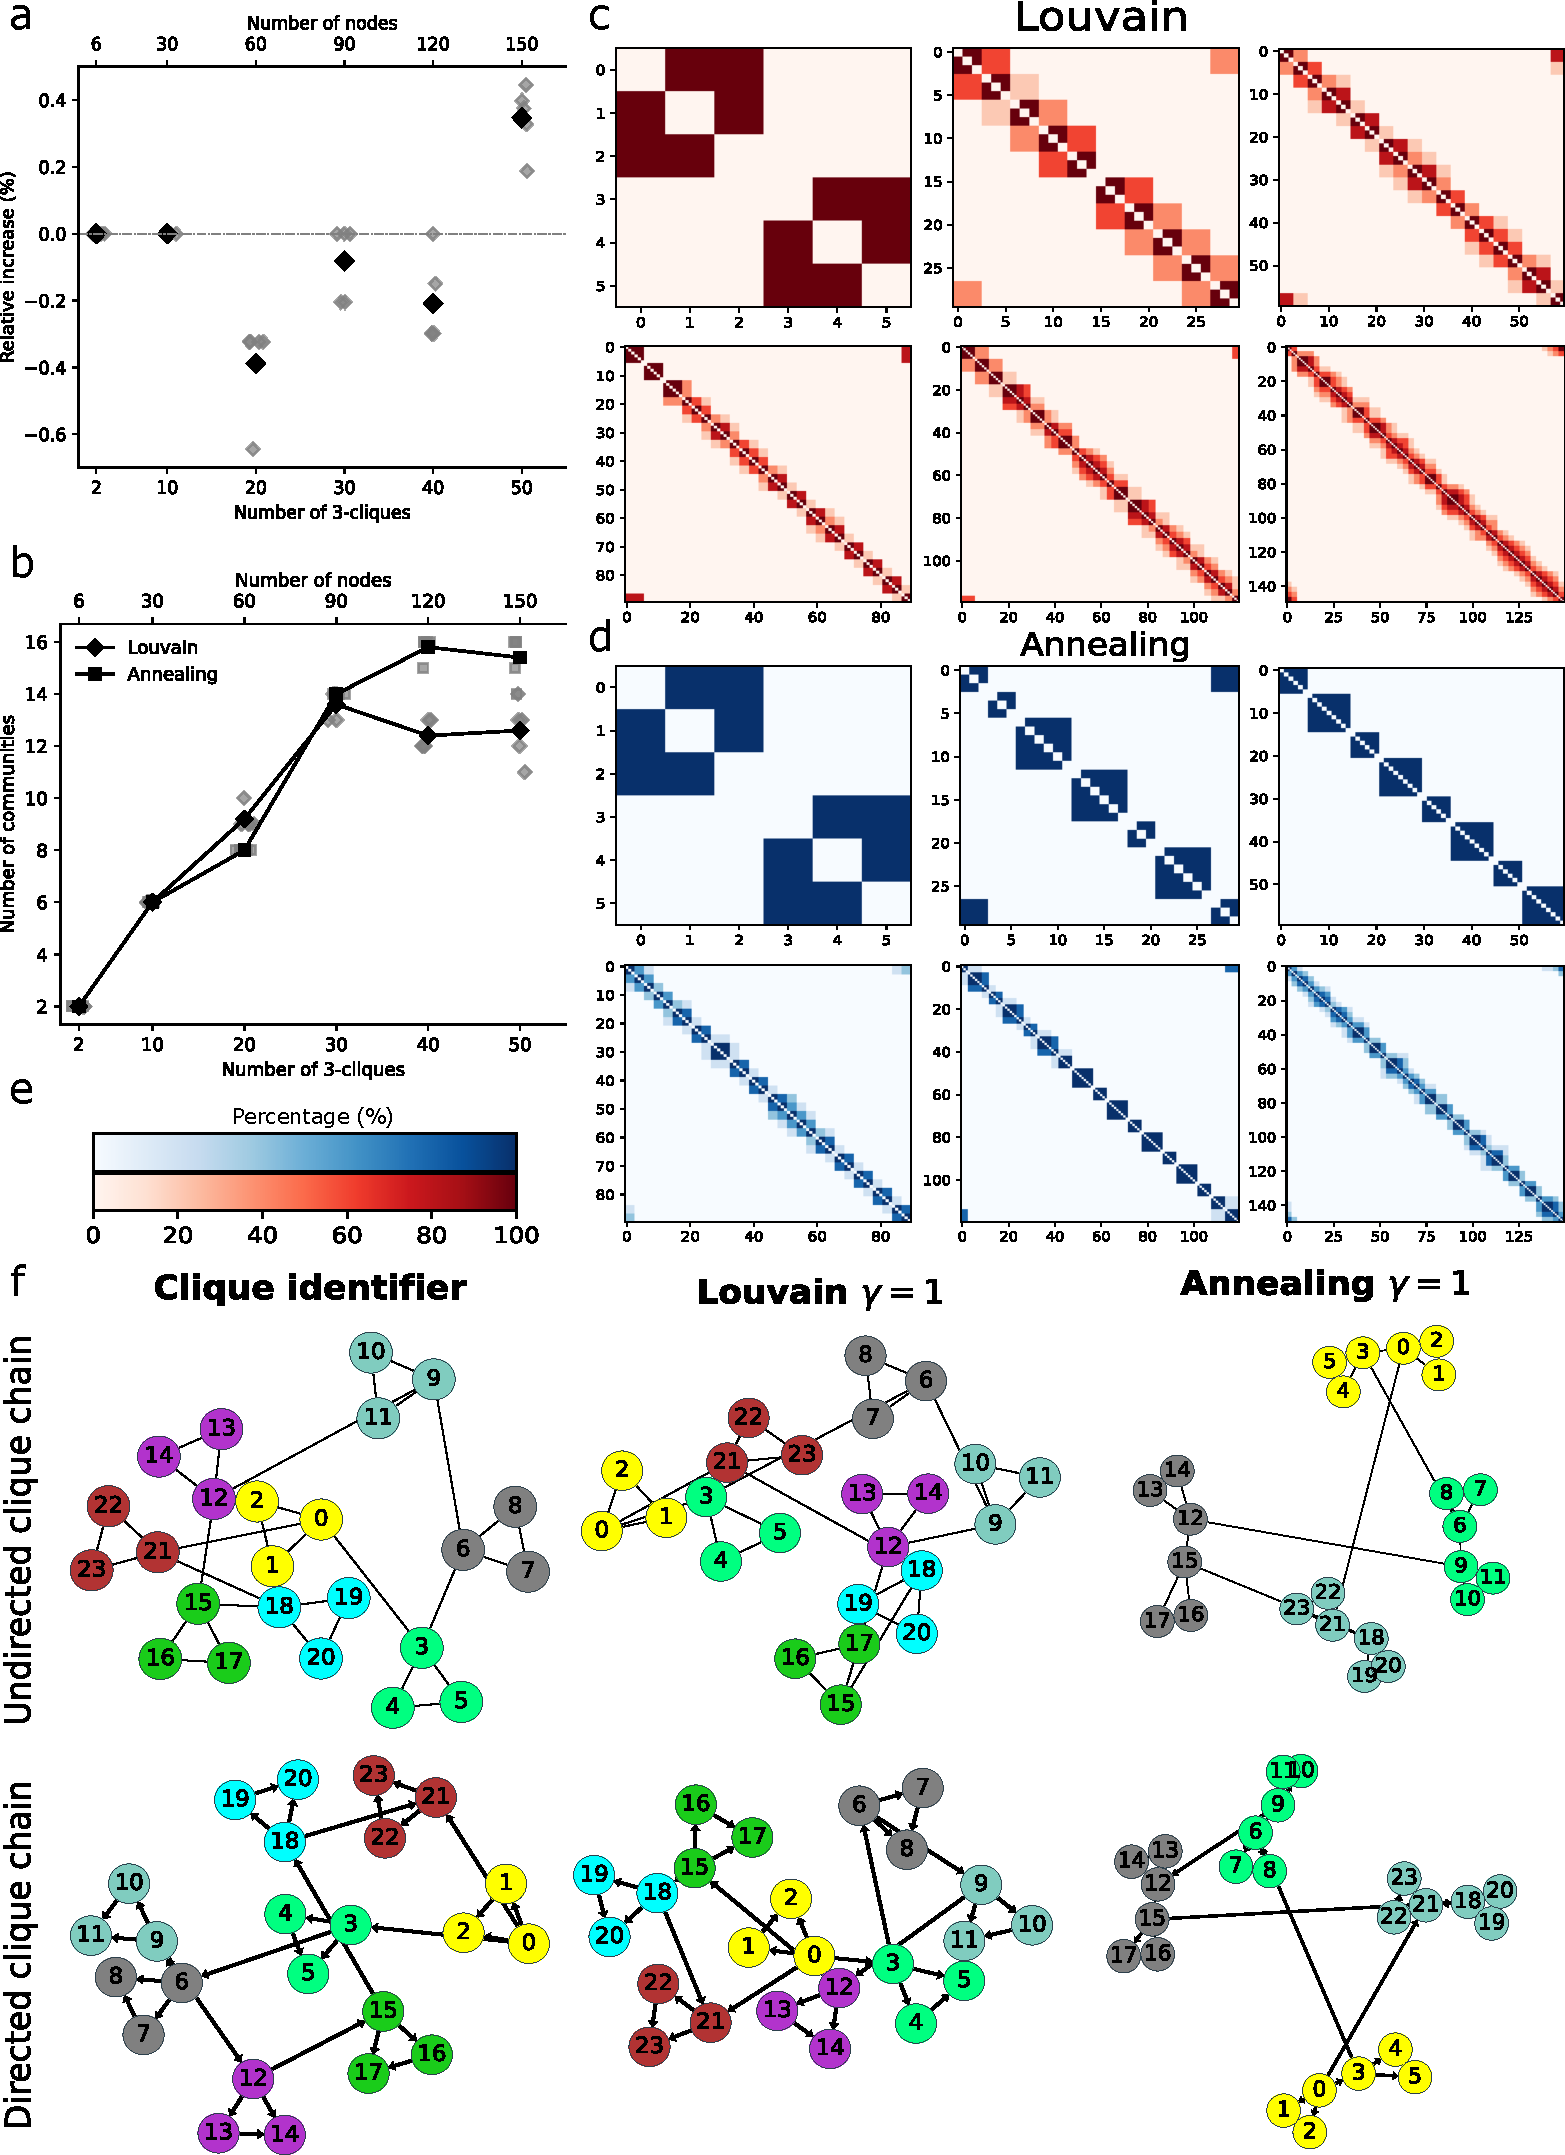
\includegraphics[width=.9\linewidth]{Figures/Fig1.pdf}
    \caption{\textbf{Communities detected with Annealing and Louvain in chains of 3-cliques.} \textbf{a} Modularity of the community structure found by the two algorithms measured as the relative increase (\%) w.r.t. the Louvain solution. Individual points (in gray) and the mean increase (black diamonds). \textbf{b} Number of communities found with each algorithm. \textbf{c, d} Consensus matrices constructed with 5 different runs for each clique chain. \textbf{e} Percentage colorbar in \textbf{c} and \textbf{d}. \textbf{f} Output of the two algorithms and the generated graph (left) for a chain of 8 3-cliques. Both the Louvain and the hierarchical annealer solutions have the exact modularity.}
    \label{fig:clique-chains}
\end{figure}

The next example is the Zachary Karate Club network \cite{zachary1977information}, a well-known dataset encoding social interactions. The current agreement, for this system describes 4 communities with a maximum modularity of 0.44904 for $\gamma=1$ (Table \ref{tab:karate}). As opposed to the clique chains studied before, the topological and geometrical structure of this network does not suggest a well-defined hierarchical structure, thus not explicitly favoring the recursive nature of our solution. We also tested a recent quantum-classical hybrid \cite{Wierzbinski2023}, known to correctly resolve this network. Noteworthy, the network is undirected and weighted, and the solution obtained through pure Hierarchical quantum annealing is entirely equivalent.

\begin{table}[h]
    \centering
    \begin{tabular}{l||c|c|c|l}
        \textbf{Algorithm} & \textbf{Max} $\mathbf{Q}$ & \textbf{Frequency} (\%) & \textbf{Number of communities} & \textbf{Time} (s) [mean $\pm$ SEM]\\
        \hline
        \textit{H. annealing} & 0.444904 & 100 & 4 & 8.46 $\pm$ 0.26 \\
        \textit{H. Gurobi} & 0.444904 & 100 & 4 & 0.110 $\pm$ 0.002 \\
        DQM & 0.444904 & 100 & 4 & 12.80 $\pm$ 0.04 \\
        Louvain & 0.444904 & 40 & 4 & 0.0037 $\pm$ 0.0004 \\
        Leiden & 0.444904 & 100 & 4 & 0.00248 $\pm$ 0.00008 \\
        Bayan & 0.444904 & 100 & 4 & 2.04 $\pm$ 0.06 \\
    \end{tabular}
    \caption{\textbf{Modularity of the Karate club network.} Maximum modularity resulting from the different algorithms tested. The maximum and frequencies are taken from a pool of 50 independent runs (see Methods). For the quantum-based solvers, the times include the embedding of the QUBO, its caching, and the communication with the D-Wave servers. In italics, we highlight the methods that directly stem from our algorithm.}
    \label{tab:karate}
\end{table}

\subsection*{Hierarchical annealing as a function of network topology}
We studied the performance of the proposed annealing process as we varied the geometry and the topology of the networks. We evaluated the solutions of the Louvain, Leiden, Bayan, and hierarchical annealing algorithms for 3 different complex types of networks and number of nodes. The quantum-classical hybrid algorithm was omitted due to its high consumption of computing minutes. A similar argument holds for Hierarchical Gurobi and Bayan, where external computational resources were needed to be acquired. 

The first networks were generated following preferential attachment and triad formation steps \cite{Holme2002}. This generates a network with scale-free and/or power-law properties, high clustering, and a good modular organization as the size of the network is increased. The number of edges to add and the probability of performing a triad formation step were kept at 1 and 0.1 respectively for all the sizes. Hierarchical annealing displayed a robust, optimal, and highly congruent behavior when compared to the other algorithms (Fig. \ref{fig:random-nets}a).

Then, we generated networks using only preferential attachment (i.e., without triad formation) \cite{Barabasi1999}). However, depending on the number of edges added at each step, the final network may or may not display a modular organization. To test the robustness of hierarchical annealing to discover communities in potentially modular networks, we kept the aforementioned parameter equal to 40\% of the network size. This generated poorly modular systems but without random topologies. For these non-trivial networks, our method remained competitive across sizes largely surpassing the Leiden algorithm (Fig. \ref{fig:random-nets}b).

We also tested the hierarchical annealing process in random networks \cite{erdds1959random}, where the probability of two nodes being connected is uniform. The topology of Erd\H{o}s-R\'enyi networks has been well characterized and is considered a valid null system for multiple graphs and topological metrics in biological systems. Again, our solution produced comparably optimal solutions for all algorithms (Fig. \ref{fig:random-nets}c). 

Finally, we studied the performance of the hierarchical quantum annealing solution in directed scale-free networks generated using the preferential attachment mechanism \cite{bollobas2003}. Again, our solution resulted in high-quality community structures for multiple network sizes (Fig. \ref{fig:random-nets}d), and even in important increments in certain cases w.r.t. the classical benchmarks (Fig. \ref{fig:random-nets}e).

\begin{figure}
    \centering
    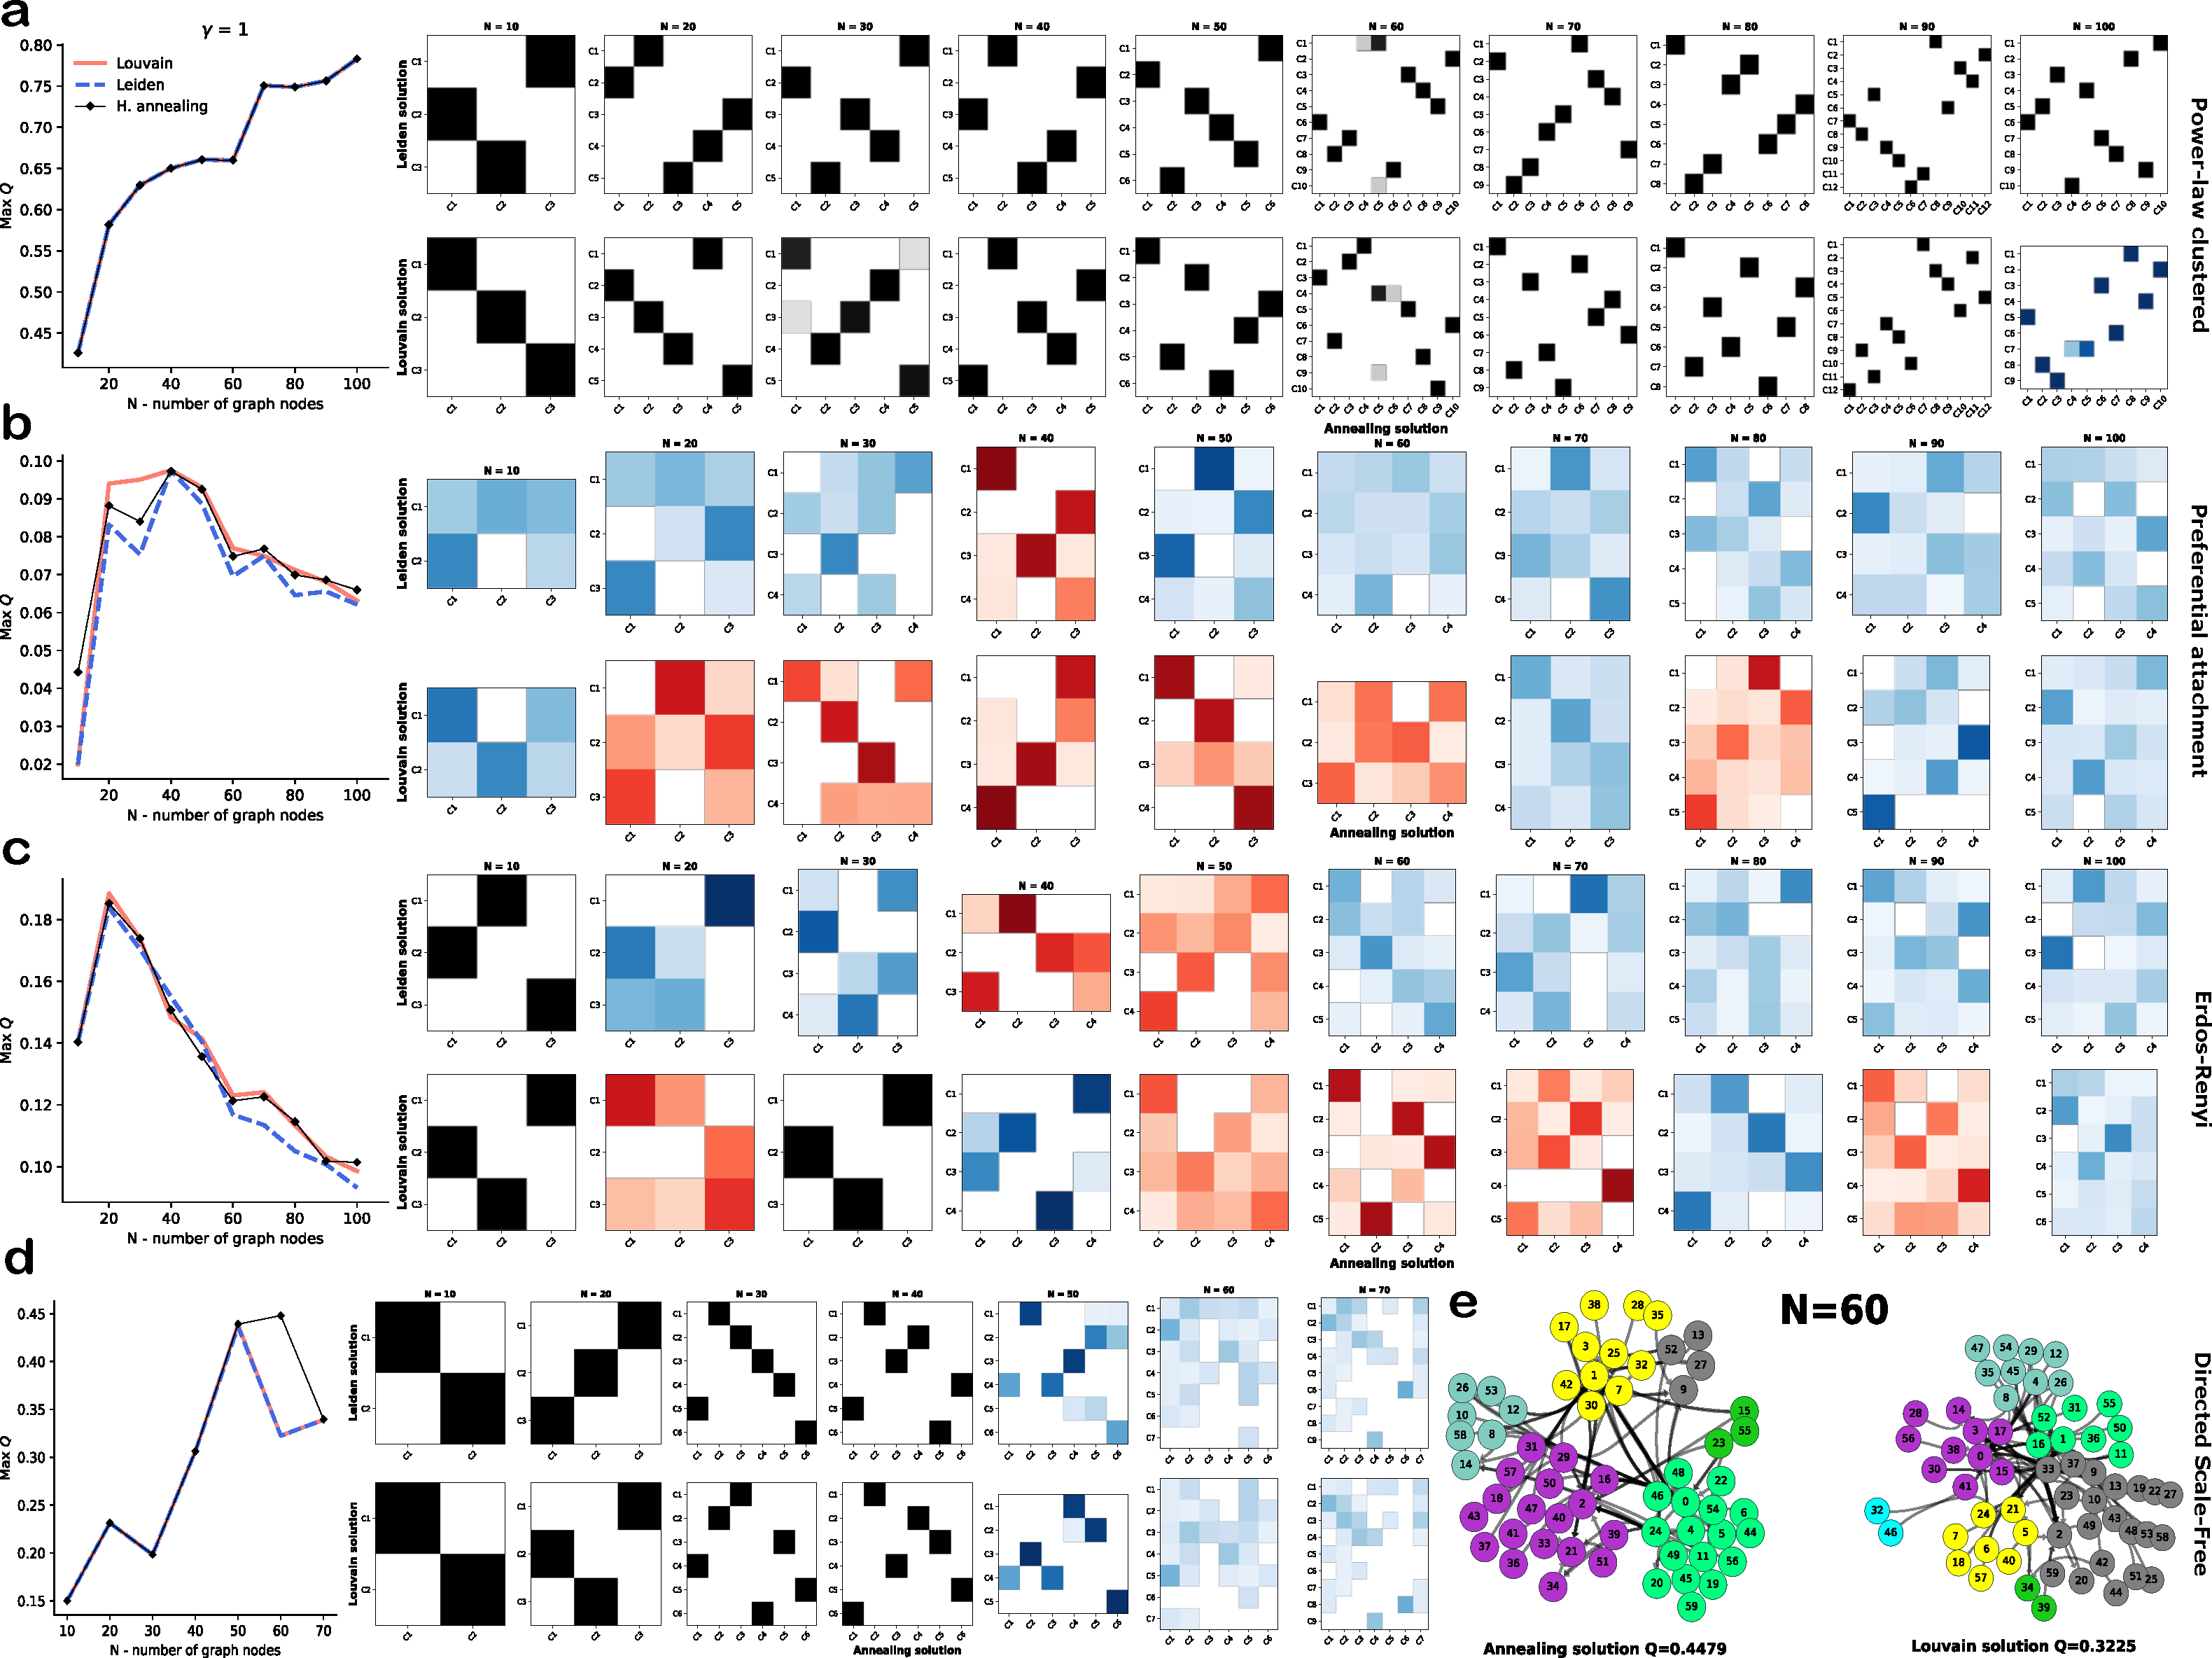
\includegraphics[width=1\linewidth]{Figures/Fig2.pdf}
    \caption{\textbf{Annealing solutions for different random networks of increasing size.} Modularity of a random network as found by the Louvain, Leiden, and Hierarchical annealing algorithms. The resolution, $\gamma$, was set to 1. To measure the overlap between the different solutions, we show the Dice score between all the communities found. The colormaps indicate if the annealing solution has a higher (in blue), equal (in black), or lower (in red) modularity. The opacity is directly proportional to the magnitude of the Dice score between each pair of communities. The random networks have been generated via the mechanisms of (\textbf{a}) power-law clustering, (\textbf{b}) preferential attachment, and (\textbf{c}) random edge creation. \textbf{d} Exact same layout for a directed scale-free network. \textbf{e} Community structure of a directed scale-free network of 60 nodes discovered through the H. annealing and Louvain algorithms. This corresponds to the network where the annealing solution was significantly superior in \textbf{d}.}
    \label{fig:random-nets}
\end{figure}

To further study the robustness of the quantum solutions, we studied the behavior of the hierarchical annealing process as a function of the power-law exponent. For that, we generated multiple networks of different sizes following the preferential attachment mechanism described previously, each one with significantly different power-law structures, and potential hierarchies (see Methods). We compared the hierarchical annealing process against the Louvain and Leiden algorithms finding very similar solutions in terms of the modularity index. Even more, the solutions showed the same inverse relationship on the power-law structure as the classical counterparts (Fig. \ref{fig:topology}a). 

More specifically, the hierarchical annealing process yielded 3 out of 36 equally optimal solutions, 16 out of 36 higher modularity scores, and 13 out of 36 worse solutions (Fig. \ref{fig:topology}b). We found that the quantum alternative tended to return more optimal solutions for networks with medium-big size and smaller power-law exponents. Therefore, we fitted a bilinear model using an ordinary least squares procedure to explain the relative increase $(\%RI)$ of the quantum solution as a function of both parameters, $$ \%RI \sim 1 + \alpha + N,$$ where $\alpha$ denotes the power-law exponent, and $N$ is the number of nodes. This model carried explanatory power ($R^2=0.3680$, $p=0.0080$, $F$-statistic against a constant model, AIC=118.2572) and both coefficients significantly contributed to the prediction ($\alpha$: $ p=0.0.0116$, $N$: $ p=0.0462$). Additionally, we included an interaction term of the form $\alpha N$. This alternative model showed a slightly higher coefficient of determination ($R^2=0.3869$, $p=0.0144$, $F$-statistic against a constant model, AIC=119.5288) but the individual coefficients were non-significant ($\alpha$: $ p=0.0863$, $N$: $ p=0.7353$, $\alpha N$: $p=0.4416$), suggesting that independent rather than interaction effects better explain the performance of the algorithm. 

To visualize and confirm these trends, we fitted two independent linear models for each parameter. The coefficient of the power-law exponent maintained the significance, while the coefficient of the number of nodes didn't despite the increasing trend in the relative increase (Fig. \ref{fig:topology}c). For scale-free networks (i.e., $\alpha \in [2,3]$), all the hierarchical annealing solutions were either superior or equivalent to ones found by the classical counterparts (Fig. \ref{fig:topology}c, green shaded area). Importantly, we only considered solutions with a relative increase and power-law exponent that fell within the 95\% range (i.e., $|z_{score}|<1.96$). Using this criteria, 4 solutions out of 36 were discarded. Crucially, 3 out of these 4 outliers, corresponded to extremely high power-law exponents.

\begin{figure}
    \centering
    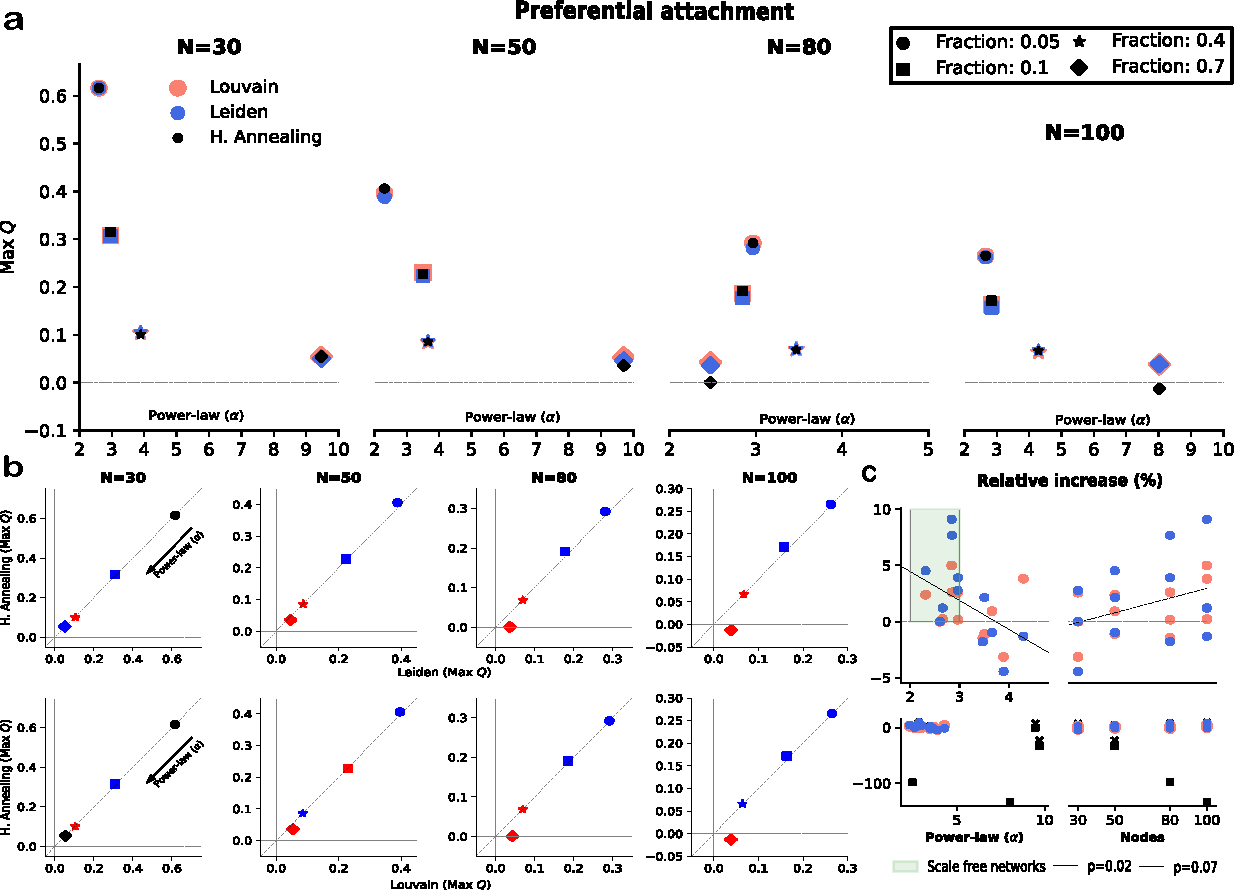
\includegraphics[width=1\linewidth]{Figures/Fig3.pdf}
    \caption{\textbf{Hierarchical annealing as a function of inherent hierarchies in the network.} \textbf{a} Modularity of the solution for the Leiden, Louvain, and Hierarchical annealing algorithms as a function of the number of nodes and scale-freeness of the networks. The networks were generated using a preferential attachment mechanism \cite{Barabasi1999}. \textbf{b} Explicit comparison between the Hierarchical annealing and Leiden (top) and Louvain (bottom) solutions on the plane. Black markers (located on the dotted diagonal line) correspond to identical solutions, blue markers correspond to better solutions from the annealer, and red markers indicate worse performances than the classical counterparts. The shape of the markers follows the top-right legend in panel \textbf{a}. \textbf{c} Relative increase of the quantum solutions in \textbf{a}, \textbf{b} as a function of $\alpha$, and the number of nodes. The green shaded area (top-left) indicates scale-free networks. The solutions in black markers (bottom) were discarded for the regression analyses.}
    \label{fig:topology}
\end{figure}

\subsection*{Hierarchical annealing for different resolution parameters}

The binary hierarchical formalism we developed in the Methods, explicitly incorporated the resolution parameter $\gamma$ in the function to optimize, as opposed to earlier accounts, classical \cite{Newman2006,Leicht2008} and quantum \cite{Ushijima-Mwesigwa2017,Negre2020}. Briefly, the process was formally independent of $\gamma$, which only appeared in the calculation of the modularity matrix (see Methods). We generated 3 different networks with nodes $N=10, 50, 80$ using preferential attachment and triad formation steps to test whether the framework returned an optimal community structure. We then ran our Hierarchical annealing procedure for different values of the resolution parameter. 

The overlap between the different solutions was consistently close to 1, and never below 0.8, as measured with the average Dice score between all the communities (Fig. \ref{fig:resolution}a). This overlap, as expected, co-varied with the number of communities found. Furthermore, the performance was stable across the range of $\gamma$ studied, showing some slight increases and decreases for individual cases (Fig. \ref{fig:resolution}b-c). 

We kept track of the total computing time for the hierarchical process to finish (see Methods). This time increased rather monotonously with the resolution (Fig. \ref{fig:resolution}c). However, larger values of $\gamma$ are related to smaller communities \cite{fornito2016fundamentals}, thus the number of calls to the QPU also increased (Fig. \ref{fig:resolution}).

\begin{figure}
    \centering
    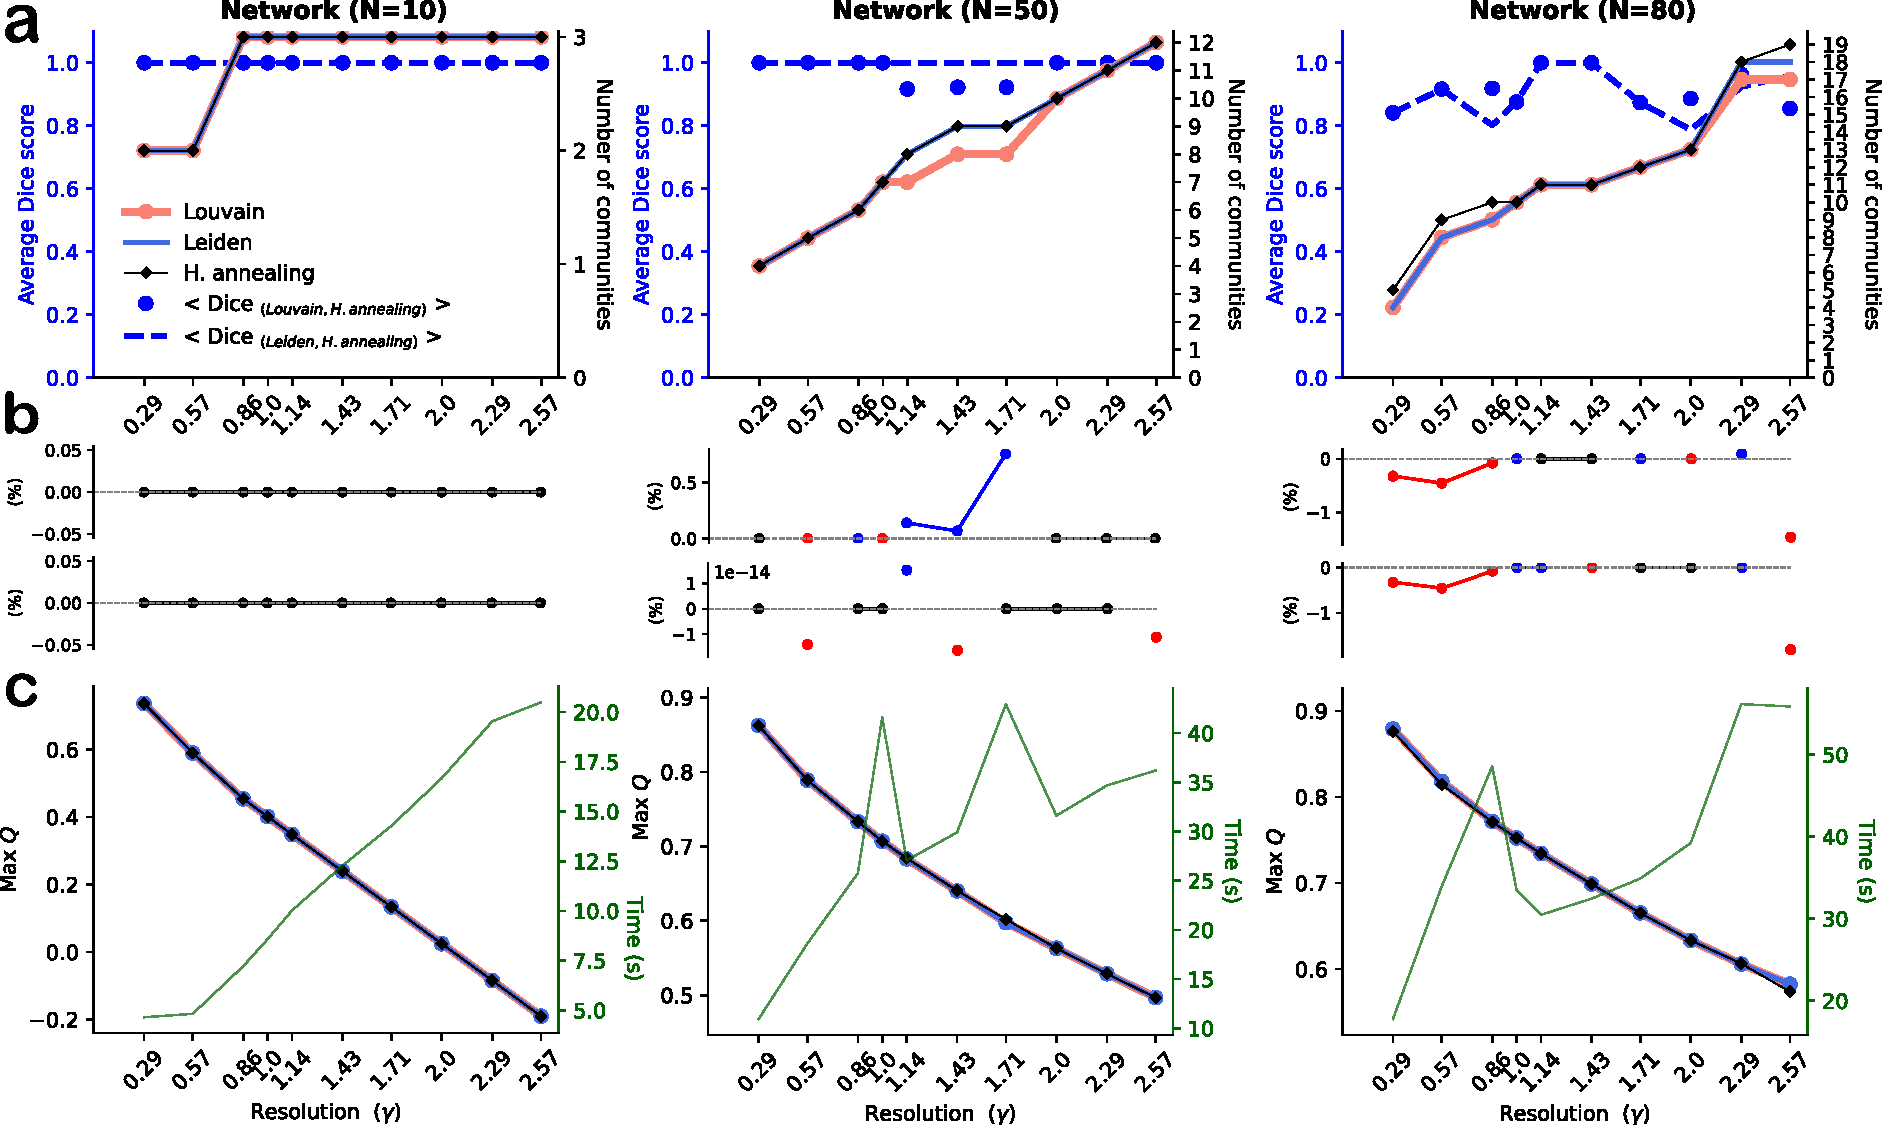
\includegraphics[width=1\linewidth]{Figures/Fig4.pdf}
    \caption{\textbf{Hierarchical annealing in different clustered power-law networks for different resolution parameters.} Each column depicts the results described below for a network of $N=10, 50, 80$ nodes respectively. \textbf{a} Measure of the average overlap between the communities found by the Louvain and Hierarchical annealing algorithms (left axis, blue) and the number of communities (right axis, salmon and black) as a function of the resolution parameter $\gamma$. \textbf{b} Relative increase of the Hierarchical annealing measured w.r.t. the Louvain (top) and Leiden (bottom) solutions in \textbf{a}. Black markers correspond to identical solutions, blue markers correspond to better solutions from the annealer, and red markers indicate worse performances than the Louvain alternative. \textbf{c} Maximum modularity per resolution value (left axis, same legend as in \textbf{a}) and the total computing time per solution (right axis, green).}
    \label{fig:resolution}
\end{figure}

\subsection*{Application of QA to structural brain connectivity}
One of the main advantages of our proposal is that we could inspect the output process at every step of the process. We plotted the modularity and the community structure in the form of a \textit{dendrogram}. The final division was dependent on each earlier subdivision, thus being interpretable as a hidden community structure. Such hidden structures would be informative of certain network vulnerabilities or strengths. We applied this visualization technique to all the networks studied up until now, while comparing the modularity of the final community structure with the same benchmark methods achieving competitive and identical results (Fig. \ref{fig:dendro_pw}; see also Supplementary Figures).

\begin{figure}[h]
    \centering
    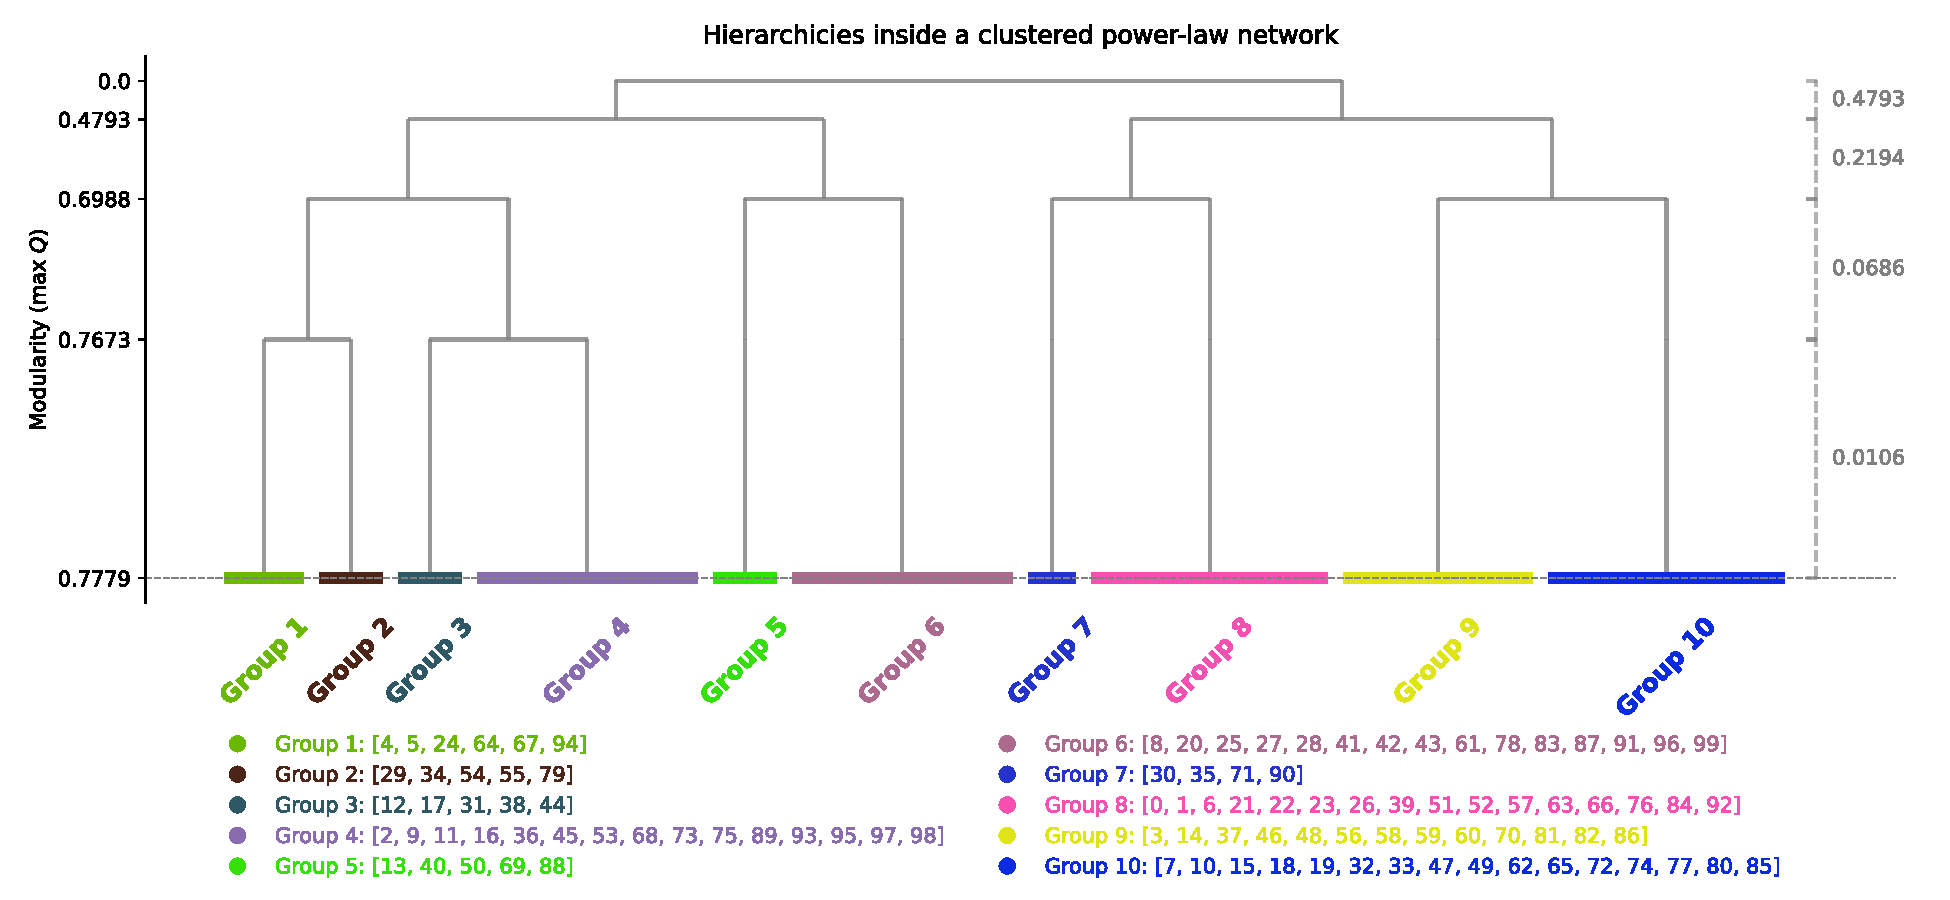
\includegraphics[width=1\linewidth]{Figures/Fig5.pdf}
    \caption{\textbf{Dendrogram of a clustered power-law network \cite{Holme2002} of N=100 nodes.} Hierarchical structure found by the H. annealing algorithm. The hierarchy corresponds to the one unraveled after maximizing the modularity of the network as described in the main text; that is, {\tt num\_runs = 15} and {\tt resolution = 1}. Both the Louvain and Leiden algorithms returned a maximum modularity of $Q=0.7779$. The left axis shows the modularity at each step of the process, while the right axis displays the corresponding increments. The bottom-most row represents the final output of the H. annealing algorithm.}
    \label{fig:dendro_pw}
\end{figure}

As a last proof of concept, we analyzed real brain connectivity networks as derived from diffusion-weighted magnetic resonance imaging methods. These networks contained a total of 166 nodes and were densely connected while exhibiting somewhat scale-free structures \cite{falco2024functional}. We also inspected the anatomical positioning and organization of the found community structure as well as the hierarchical levels of the process (Fig. \ref{fig:dendro_aal}). Despite the large number of variables (i.e., qubits), the H. annealing solution was strikingly close to the solutions found by the Louvain and Leiden algorithms. Furthermore, the communities found by the quantum algorithm only differed slightly in the frontoparietal border, areas that are highly interconnected with U-fibers. The rest of the identified communities were largely in agreement between algorithms (see Supplementary Figures), hence setting a very promising set of baseline results for more advanced and sophisticated QA methods and algorithms.

\begin{figure}[h!]
    \centering
    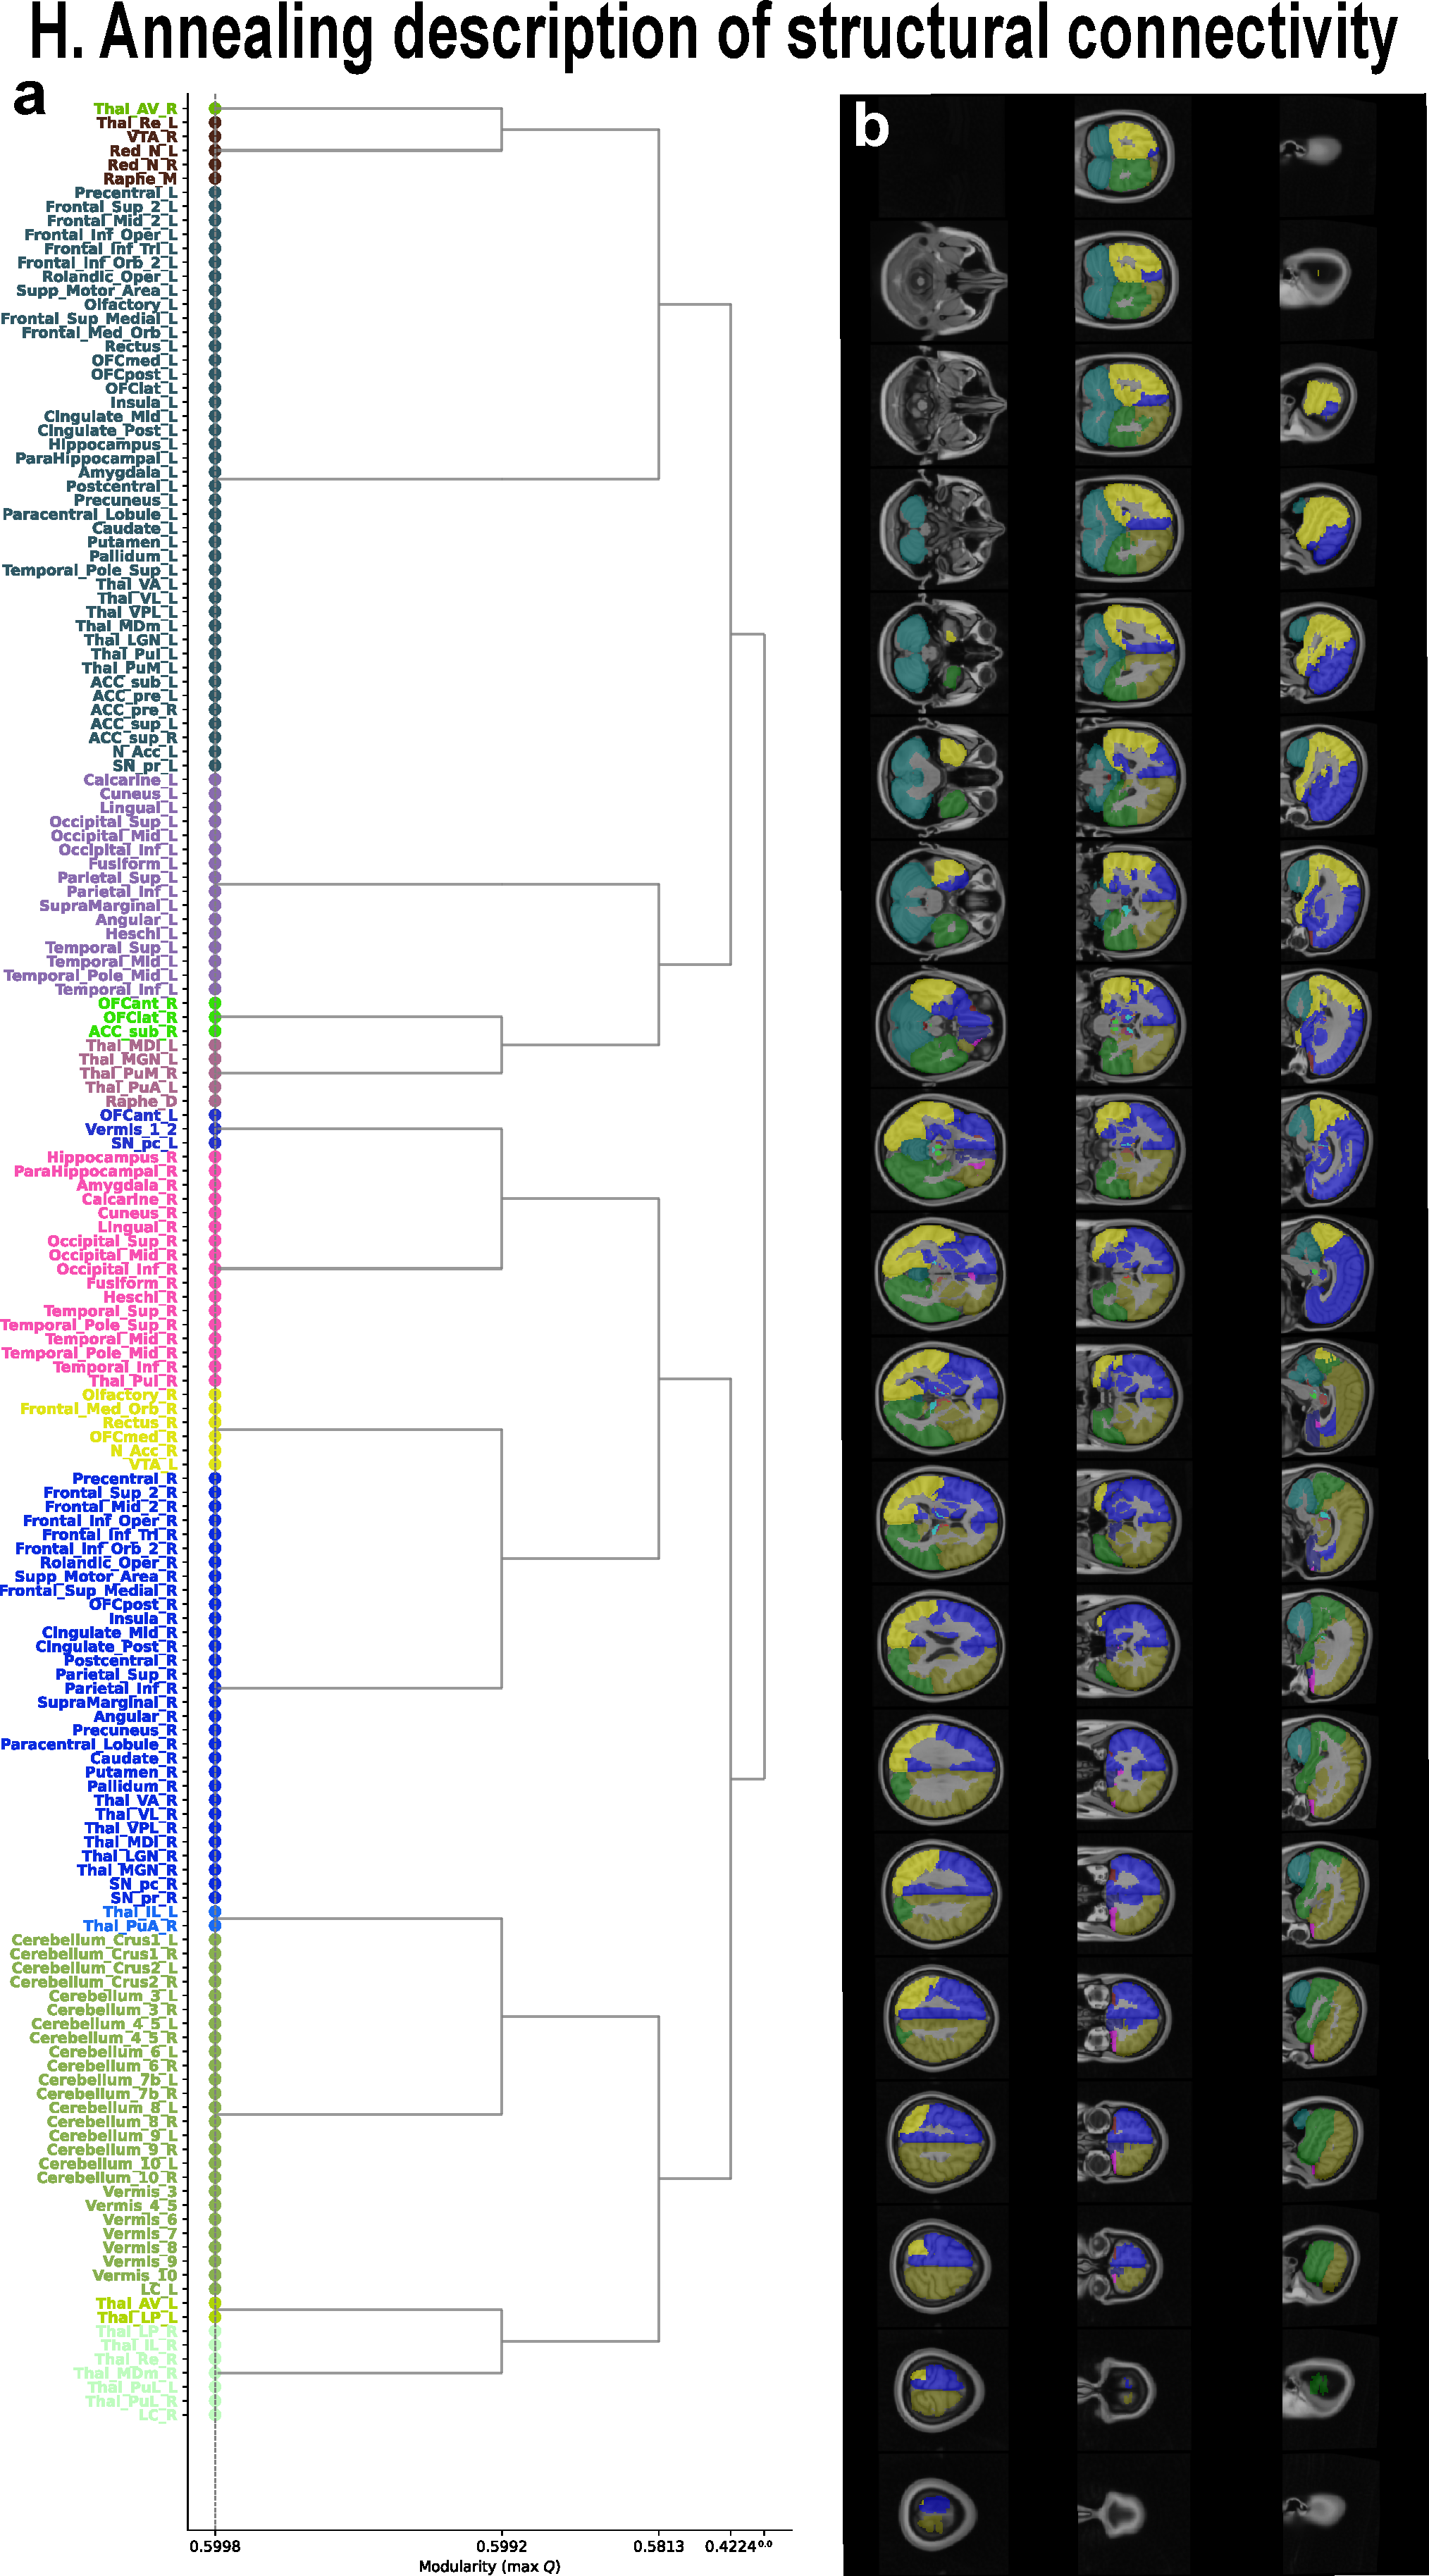
\includegraphics[width=.7\linewidth, height=19cm]{Figures/Fig6.pdf}
    \caption{\textbf{Dendrogram of a real brain structural connectivity network \cite{falco2024functional}.} \textbf{a} Hierarchical structure found by the H. annealing algorithm. The hierarchy corresponds to the one unraveled after maximizing the modularity of the network as described in the main text; that is, {\tt num\_runs = 10} and {\tt resolution = 1}. The Louvain and Leiden algorithms returned a maximum modularity of $Q=0.611$ and $Q=0.610$ respectively. The left axis shows the modularity at each step of the process, while the right axis displays the corresponding increments (i.e., Eq. \ref{eq:p_k}). The bottom-most row represents the final output of the H. annealing algorithm. \textbf{b} Overlay of the structural communities on the Montreal Neurological Institute (MNI) 152 template. Each color corresponds to a different community, whose elements can be found in \textbf{a}.}
    \label{fig:dendro_aal}
\end{figure}

\section*{Discussion} \label{sec:discussion}

Here we present a quantum approach to discovering communities in complex networks. We unify the optimization process for binary, weighted, and directed networks and explicitly consider the resolution parameter to consider multiple topological scales present in the networks. Our experiments show that quantum annealing (QA) can be successfully used to maximize the modularity of a network and pinpoint meaningful groups of highly connected nodes. Its performance is robust across multiple experimental conditions and, at least comparable to alternative methods based on classical heuristics. As opposed to earlier attempts, we restrict ourselves to pure QPUs avoiding hybrid solutions that obscure the algorithm results \cite{Negre2020,Wierzbinski2023} and provide an account of the possible origins of suboptimal performances. While many community detection algorithms rely on maximizing a quality function \cite{Fortunato2010}, not all are well-suited for every type of network. Thus, the same could be said about our proposal, which explicitly relies on the existence of hierarchies. While we show how the Hierarchical annealing process performs well in networks without a clear topological organization (Fig. \ref{fig:random-nets}, see also Table \ref{tab:karate}), we note how and why exploiting inherent hierarchies could be beneficial rather than detrimental in the study of real-life complex systems. 

\subsection*{Unveiling hierarchies in complex networks with quantum computing}
Biological and social networks are dynamic rather than static systems, even if we study their properties at a fixed point in time. Their evolution is thus constrained to the underlying mechanism that governs the interactions between their constituents. Barabasi and Albert \cite{Barabasi1999} showed that preferential attachment, where highly connected nodes attract more links, leads to scale-free networks with a slower decay of highly connected nodes than in random networks. Preferential attachment can lead to structural hierarchies, but the latter is not guaranteed \cite{Holme2002,barabasi2003scale}. Furthermore, life processes themselves are hierarchical \cite{oltvai2002life,alon2003biological}, inspiring specific methods to discover such organization \cite{SalesPardo-etal_2007}. In neuroscience, brain network structure is influenced by plasticity mechanisms occurring across temporal and spatial scales. Hebbian plasticity, in particular, has been shown to modulate preferential attachment, resulting in scale-free and clustered network structures \cite{Lynn2024}. It is therefore not unreasonable to assume some underlying hierarchical structure to design the algorithms. In the context of our work, we show how the Hierarchical annealing process performs exquisitely in these kinds of systems even improving over classical alternatives (Fig. \ref{fig:topology}). Additionally, network size did not significantly affect performance, suggesting the process is robust and scalable. The slightly suboptimal results we observed likely stem from the hierarchical process itself \cite{Arenas2008}, rather than issues with the annealing steps given that we mitigated its variability by using multiple and independent instances of the quantum hierarchical process. 

One of the main advantages of the hierarchical approach we studied, is the direct interpretability of each one of the recursive divisions. We can construct \textit{dendrograms} of the sequence of divisions that yield the highest modularity indices for any given network. However, the correctness of such dendrograms depends entirely on the optimality of the represented solution. For that, it remains essential to compare the modularity of the community structure with solutions from other algorithms. As expected, the obtained using H. annealing for all the networks studied in this work were extremely competitive, thus offering insights into the hidden structure of these networks (Figs. \ref{fig:dendro_pw} and \ref{fig:dendro_aal}; see also Supplementary Figures). There exist some attempts to reveal hierarchies present in complex networks, most notably relying on bottom-up hierarchical clustering methods \cite{SalesPardo-etal_2007,Arenas2008} and the combination of resolution parameters \cite{lambiotte2013multi}, therefore offering a complementary rather alternative description of fractal-like structure. A few other methods have been developed using the Louvain algorithm to unravel hierarchical relationships within complex systems. For example, each iteration of the Louvain algorithm can be interpreted as a step in a hierarchical process \cite{Blondel2008,meunier2009hierarchical}. Alternatively, separate instances of the Louvain algorithm may be used to discover community structures within sub-modules \cite{bassett2010efficient}. Instead, our approach considers the whole system at each step inside the hierarchy \cite{Newman2006,Leicht2008} (see also Eq. \ref{eq:p_k}). Because of that, and contrary to the Louvain solution, this guarantees that every step in the hierarchy is divided taking into account the whole system rather than local sub-modules, a desirable feature for strongly nested systems where our method is expected to outperform several alternatives (Fig. \ref{fig:topology}; see also Supplementary Figures).

\subsection*{Towards quantum-based multi-resolution community detection methods}
The specific case where the resolution parameter $\gamma$ is 1, for which we recover known results in the literature \cite{Newman2006}, simplifies several expressions throughout this work. However, discovering communities via maximizing the modularity function possesses an inherent limitation where communities smaller than a given size are likely to be omitted \cite{Fortunato2007}. Kumpula, \textit{et al.}, proved that this limit persisted for all $\gamma$ independently of the null model used in the definition of $Q$ \cite{Kumpula2007}. Although the resolution parameter was introduced to weigh the topological scale at which communities ought to be detected \cite{Reichardt2006}, it was elegantly shown that it could be employed to overcome the resolution limit \cite{Traag2011}, albeit disregarding the null model (e.g., $\frac{g_ig_j}{2m}$). Consequently, approaches that use different definitions for modularity function and the parameter $\gamma$ also exist \cite{reichardt2004detecting,raghavan2007near,Arenas2008,ronhovde2010local}. However, they still fall within spin-glass systems, therefore being possible to tackle using the same formalism we used. 

Nonetheless, Newman and Girvan's quality index \cite{Newman-Girvan_2004} along with the explicit inclusion of a resolution parameter \cite{Reichardt2006}, remains, up to date, the most common choice for discovering community structure but, unfortunately, the exact value remains, up to date, an arbitrary choice. In short, large values of the resolution will yield smaller communities, while smaller values of $\gamma$ will result in fewer communities of increased size. Hence, we root the parameter $\gamma$ inside our framework for two main reasons: 1) users need not tune the objective function to maximize, and, 2) it easily adapts to multiresolution methods. We maintain $\gamma$ as a free parameter and we derive all our expressions without specifying its value. Our experiments using multiple values of $\gamma$ within a meaningful range show that the Hierarchical annealing process is robust w.r.t. the chosen resolution; even in networks without inherent hierarchies (Fig. S1). This feature allows us to speculate that QA can effectively detect community structure using multiresolution methods, where $\gamma$ is gradually changed or sampled nonuniformly along the optimization process \cite{Jeub2018}. Further work should address whether this holds or not, the range for which the annealer cannot coordinate the large number of communities found, and the computational time required to obtain the large number of relatively small-size communities expected for $\gamma > 3$.

Quantum processing units (QPUs), regardless of type, are known to struggle with encoding large numbers of variables. In one-hot encoding, this number is of the order $N\times M$ where $N$ is the number of nodes in the graph and $M$ is the number of allowed communities. This is suboptimal because there is no guarantee that the network contains $M$ distinct communities, leading to wasted computational resources \cite{Negre2020}. Our approach, by contrast, limits the number of variables to the size of the network. Additionally, our method optimizes systems using discrete rather than binary variables, offering another advantage. Current approaches using one-hot encoding require satisfying a constraint for each variable, $\sum_{j=1,M}x_{ij}-1=0, \ \forall i=1, \ldots, N$, which ensures each node is uniquely assigned to a community. These constraints are typically relaxed by introducing Lagrange $\alpha_i$ multipliers in the QUBO formulation. However, determining appropriate values for these multipliers often requires manual tuning or guessing, a process that becomes impractical for weighted networks, where even slight variations can alter the optimal value. While constrained optimization methods can be effective \cite{Ushijima-Mwesigwa2017,Negre2020}, they add a layer of complexity. An alternative approach, discrete quadratic modeling with hybrid quantum-classical methods, offers a promising compromise \cite{Wierzbinski2023} but sacrifices transparency. Although we employed a recursive process, other combinations of multiple binary divisions could be designed to tackle this and other optimization problems \cite{Nembrini2022}, potentially leading to quantum-classical algorithms similar to the Louvain method. For example, in \cite{rathore2024loadbalancinghighperformance}, a similar hierarchical approach is used to divide the graph of data points into $2^n$ equal parts to achieve load balancing for parallel processing.

\subsection*{Limitations and future work}
A limitation of this work is the increased computational time compared to classical heuristics. However, simulated annealing returns very good results at the cost of increased computational times \cite{Guimera2004}. Our preliminary experiments suggest a roughly linear relationship between the number of communities detected and the elapsed time. Some observed irregularities in timing may be due to repeated instances and calls to the QPUs. Although we mitigated this by caching precomputed graph embeddings, we were unable to fully address the causes of these longer times. While total times never exceeded one minute per network per run, this remains a limitation for larger, highly segregated networks. Notably, the average time consumed by the QPU per binary division, as reported by the D-Wave portal, was approximately 2 milliseconds, comparable to times for the Louvain and Leiden methods. Thus, with further research, quantum annealing and its combination with algorithmic processes could potentially become competitive in this regard while increasing its accuracy.

Lastly, we did not include signed networks in our formalism, but the extension to them represents a crucial step prior to the general acceptance of QA for the discovery of community structure. Signed networks can contain weighted, negative, and directed networks which make their study an active field of research. Although these networks allow the same spin-glass description used throughout this work \cite{Traag2009}, some definitions are tailored to each scientific discipline \cite{Kaplan2008,Gomez2009,rubinov2011weight}. This calls for specific rather than generic descriptions of the function to optimize, something that we wanted to avoid here. However, it is necessary to assess the performance of QA in these types of systems where non-trivial interactions can emerge (e.g., frustration \cite{kirkley2019balance}).

\subsection*{Conclusions}
In this work, we use the D-Wave Advantage annealer to maximize the modularity function to discover community structure in complex networks. We demonstrate that hierarchically dividing the network and, at each step, optimizing a binary problem effectively eliminates the need to use one-hot encoding and constraints to maximize Newman's quality function. As opposed to earlier attempts, the number of communities can be left uncontrolled and found by the algorithm. Moreover, extending Newman's ideas \citep{Newman2006,Leicht2008}, we analytically show how the function to maximize remains formally independent from the resolution parameter and whether the network is undirected, directed, and/or weighted. We thoroughly conduct experiments to assess whether the underlying topology of the network represents a liability to this nested approach finding that the pure quantum process is stable across topologies and even performs better in scale-free networks, which are ubiquitous in biological systems. Furthermore, the same procedure could, in principle, be applied for multiresolution clustering purposes in any given type of network given that the Hierarchical annealing optimization remains largely equivalent to classical counterparts for multiple values of the resolution parameter. Lastly, the hierarchical annealing process we present allows for interpretable results. When adequately compared to classical alternatives, it permits the exploration of hidden hierarchies within complex systems, potentially indicative of several network dysfunctions.  

\section*{Materials and methods} \label{sec:methods}
\subsection*{Modularity index and quantum annealing}
A graph or network $G=(V,E)$ is a set of vertices or nodes $V$ and edges $E$. Moreover, a community in the graph is a subset of nodes $c\subseteq V$. A community structure is a set of non-overlapping communities $C=\{c_r | c_r \subseteq V, c_s \cap c_r=\varnothing, \text{ for } s \neq r \}$. The set of all possible community structures is denoted as  $\mathcal{C}$. Importantly, a community is not a subgraph as it doesn't require the deletion of inter-community edges. Lastly, the quality of a given community structure $C$ can be quantified with the modularity index \cite{Newman2004},
\begin{equation} \label{eq:modularity}
    Q = \sum_{c \in C}\left[ \frac{L_c}{m} - \gamma \left(\frac{d_c}{2m}\right)^2\right],
\end{equation} where $L_c$ is the number of links between nodes in the $c$-th community, $d_c$ is the sum of the degrees of those nodes, and $m$ is the total number of links (or edges) in the network. Moreover, $\gamma$ is a resolution parameter that effectively accounts for different topological scales \cite{Reichardt2006} at which interactions between nodes happen \cite{Delvenne2010}.

A certain community structure is said to be modular if it exhibits a high modularity index when compared to multiple random instances of a given class of random networks (e.g., Erd\H{o}s-Renyi). Community detection algorithms aim to find a given community structure $C \in \mathcal{C}$ whose associated modularity function $Q$ lies at a global maximum -- or its opposite at a minimum, 
\begin{equation}\label{eq:min_mod}
    \hat{Q} \doteq \max_{\forall C \in \mathcal{C}} \left[Q\right] = - \min_{\forall C \in \mathcal{C}} \left[-Q\right].
\end{equation}
Even though $\mathcal{C}$ is bounded, the number of possible elements it contains grows faster than exponentially with the size of the network \cite{Fortunato2007}. Furthermore, it has been proven that maximizing modularity is an NP-complete problem \cite{Brandes2008}, thus justifying QA methods \cite{Farhi2001}. To maximize the modularity index, the first term in Eq. \ref{eq:modularity} suggests defining clusters containing a large number of edges. 
%Contrary, the second term aims that the size of such clusters should be as small as possible. 
On the contrary, the second term aims to minimize the size of such clusters.
This is important because any algorithm could be prone to isolate given nodes to artificially boost the modularity index \cite{Wierzbinski2023}.

For a network of two communities, the modularity function in Eq. \ref{eq:modularity} can be mapped into an Ising system with variables $s_i = \{-1,1\}$ indicating that a certain node belongs to either one of the two communities present in the network \cite{Newman2006,Reichardt2006,Negre2020,Wierzbinski2023}. For undirected networks,
\begin{equation} \label{eq:mod_ising_symm}
    Q = \frac{1}{4m} \sum_{ij\in G} B_{ij} s_i s_j + \frac{(1-\gamma)}{2},
\end{equation} where
\begin{equation} \label{eq:und_mod_matrix}
    B_{ij} = A_{ij} - \gamma \frac{g_i g_j}{2m},
\end{equation} are the entries of the \textit{modularity} matrix, $A_{ij}$ are the entries of the symmetric adjacency matrix, $m = \frac{1}{2}\sum_{ij \in G}A_{ij}$ is the total edge-weight, and $g_i=\sum_j A_{ij}$ is the node weighted degree. For directed networks \cite{Leicht2008},
\begin{equation} \label{eq:mod_ising_dir}
    Q = \frac{1}{2m} \sum_{ij\in G} B_{ij}^{d} s_i s_j + \frac{(1-\gamma)}{2},
\end{equation} where 
\begin{equation} \label{eq:dir_mod_matrix}
    B_{ij}^d = A_{ij} - \gamma \frac{g_i^{in} g_j^{out}}{m}
\end{equation} are the entries of the \textit{directed} modularity matrix, $A_{ij}$ are the entries of the asymmetric adjacency matrix,  $m=\sum_{ij}A_{ij}$ is the total edge-weight, $g_i^{in}=\sum_j A_{ij}$ is the node weighted in-degree, and $g_j^{out}=\sum_i A_{ij}$ is the node weighted out-degree. The superscript $d$ denotes a directed or asymmetric matrix. We detailed all the algebraic intermediate steps in the Supplementary Material. 

\subsection*{Unconstrained hierarchical binary optimization}
Let us define a process $\mathcal{P} \doteq (p_k)_{k=0}^{\infty}$ as a sequence of elements $p_k$ such that its series converges to a finite value,
\begin{equation} \label{eq:process_P}
    \hat{Q}^{\mathcal{P}} \doteq \sum_{k=0}^{\infty} p_k. 
\end{equation} Crucially, minimizing $\hat{Q}^{\mathcal{P}}$ need not be straightforward. However, sequentially optimizing each element of the process $p_k$ is entirely equivalent,
\begin{equation} \label{eq:min_process}
    \min \left[ \hat{Q}^{\mathcal{P}} \right] = \min\left[\sum_{k=0}^{\infty} p_k \right] = \sum_{k=0}^{\infty}  \min \left[ p_k \right]. 
\end{equation} Our heuristic is based on the additive nature of $Q$, where each community represents an isolated entity that independently contributes to its value \cite{Newman2004}. A natural way to exploit this property is to recursively divide communities into two \cite{Newman2006}. Therefore, 
\begin{equation} \label{eq:p_k}
    \begin{cases}
        p_k &= -\left[ Q(C^{k}) - Q(C^{k-1}) \right]\\
        p_{0} &= -Q(C^{0})
    \end{cases}
\end{equation} where $0 \leq |C^{k}| - |C^{k-1}| \leq |C^{k-1}| + 1$, and $Q(C^{k})$ is the modularity of the network after splitting a given community $c \in C^{k-1}$ into two. It is straightforward to see that $\hat{Q}^\mathcal{P} \to Q(C^{\infty})$ with $C^{\infty}$ being a community structure of arbitrary size. Thus, we wish to maximize the modularity by recursively subdividing each community into two. 

Formally, there is no guarantee that a given \textit{optimized} process will univocally yield the partition with the highest modularity index in Eq. \ref{eq:min_mod}, $\min \left[ \hat{Q}^{\mathcal{P}} \right] \to \hat{Q}$. 
However, given that the problem itself is NP-complete \cite{Brandes2008}, heuristic processes are needed. Several algorithms have been developed based on the idea that optimizing in smaller steps, rather than all at once, yields competitive results. Among these, the Louvain method is the most popular \cite{Blondel2008}. In what follows, we derive the Quadratic Unconstrained Binary Optimization (QUBO) cost function for each element of $\mathcal{P}$. We then show how following the approach described here can yield high-quality community structures of arbitrary size without having to use one-hot encoding constraints \cite{Ushijima-Mwesigwa2017,Negre2020} nor discrete variables \cite{Wierzbinski2023}.  

\subsection*{Undirected networks}
Following Eq. \ref{eq:modularity}, the modularity of an undirected network of $|C^{k-1}|$ different communities can be decomposed as 
$$ Q(C^{k-1}) = \sum_{c \in \Tilde{C}^{k-2}} \left[ \frac{L_c}{m} - \gamma \left(\frac{d_c}{2m}\right)^2\right] + \frac{L_k}{m} - \gamma \left(\frac{d_k}{2m}\right)^2 $$ where $\Tilde{C}^{k-2} \cup k = C^{k-1}$. Then, the modularity index of the same network after splitting the $k$-th community in two can also be decomposed as
$$ Q(C^{k}) = \sum_{c \in \Tilde{C}^{k-2}} \left[ \frac{L_c}{m} - \gamma \left(\frac{d_c}{2m}\right)^2\right] + \sum_{r=1}^{2} \left[ \frac{L_{k_{r}}}{m} - \gamma \left(\frac{d_{k_{r}}}{2m}\right)^2 \right]$$ where $k_1 \cup k_2 = k$. Using Eq. \ref{eq:mod_ising_symm} we obtain a compact expression for the elements of $\mathcal{P}$ in terms of the modularity matrix,
\begin{equation} \label{eq:pk_symm}
    \begin{split}
        p_k &= -\left[ Q(C^{k}) - Q(C^{k-1}) \right]\\
        &= \frac{-1}{4m} \sum_{ij \in k} \left( B_{ij}s_i s_j - B_{ij}\right) - \frac{1-\gamma}{2} \\
        &= \frac{-1}{4m} \sum_{ij \in k} \left( B_{ij} - \delta_{ij} \sum_{r\in k} B_{ir}\right)s_i s_j = \frac{-1}{4m} \sum_{ij \in k} B_{ij}^{\text{k}} s_i s_j \\
        &= \frac{-1}{m} \sum_{ij \in k} B_{ij}^{\text{k}} x_i x_j + \frac{1}{2m} \sum_{ij \in k} B_{ij}^{\text{k}} x_i + \frac{1}{2m} \sum_{ij \in k} B_{ij}^{\text{k}} x_j + \frac{1}{4m} \sum_{ij \in k} B_{ij}^{\text{k}} \\
        &= \frac{-1}{m} \sum_{ij \in k} B_{ij}^{\text{k}} x_i x_j.
    \end{split}
\end{equation} We have arbitrarily dropped the constant term $\frac{1-\gamma}{2}$ since it doesn't play a role in the optimization.  
\begin{equation} \label{eq:gen_mod_matrix}
    B_{ij}^{\text{k}} = B_{ij} - \delta_{ij} \sum_{r\in k} B_{ir} \ \ \forall i,j \in k,
\end{equation} is the generalized modularity matrix \textbf{B}\textsuperscript{k} for the $k$-th community \cite{Newman2006}, we used $s_i^2=1$, and $\delta_{ij}$ is the Kronecker delta function. In the second row, we have applied a linear mapping from the Ising variables to a set of binary ones $s_i=2x_i-1$ to obtain the QUBO formulation. The last row follows from some of the properties of the generalized modularity matrix.

Importantly, the first element of the process need not be considered separately. When $k=0$, taking into account that $x_i^2 = x_i$, it is easy to show how $p_k$ reduces to the known function to split the whole network in two,$$ p_0 = \frac{-1}{m} \left[ \sum_{ij\in G} B_{ij} x_i x_j + (1-\gamma)\sum_{i\in G} g_{i} x_i \right] = -Q(C^{0}).$$ Even more, it follows that, $$\text{if } x_i=x_j \ \ \forall i,j \in k \subset V \implies p_k = 0,$$ hence no further increment can be obtained by further subdividing the chosen community. This provides a natural stopping for the hierarchical divisions without the need to predefine a maximum number of communities, either with one-hot encoding dimensions \cite{Ushijima-Mwesigwa2017,Negre2020} or integer variables \cite{Wierzbinski2023}. In practical terms, given that the network is symmetric, the summations do need to cover all the $N^2$ entries but rather the diagonal and upper diagonal entries (i.e., $\frac{N^2}{2}$). This also speeds up the computation parts, where the QUBO problems have significantly shorter symbolic expressions (see Supplementary Material).

\subsection*{Directed networks}
If the network has some degree of asymmetry, we could proceed identically as for undirected networks. The only difference would be the usage of the expressions for directed networks in order to obtain the elements $p_k$ of the process $\mathcal{P}$ (see Supplementary Material for the full derivation) 

\begin{equation} \label{eq:pk_dir}
    p_k = \frac{-8}{m} \left[ \sum_{ij \in k} B_{ij}^{d,\text{k}} x_i x_j  - \frac{1}{2} \sum_{j\in k} x_j \sum_{i\in k} \left(B_{ij}^d - B_{ji}^d \right)\right].
\end{equation}
However, contraty to the undirected case, although $p_k$ reduces to the same expression in Eq. \ref{eq:pk_symm} if the modularity matrix is symmetric, the first element of the process does not coincide with the modularity function to optimize for the full graph (i.e., $p_0 \neq Q(C^0)$). This is undesirable (but not critical) because it would mean that the first step of the hierarchy needs to be separated from the rest. Furthermore, the symbolic expression for the corresponding QUBO problem would possess $N(N+1)$ symbolic terms, potentially compromising the computational workflow for large graphs. Lastly, the $ij$-th and $ji$-th entries would be associated with the product of binary variables $x_i x_j$. Then, the QPU would interpret the coupling of the two qubits as a sum of $B_{ij}^{d,\text{k}} + B_{ji}^{d,\text{k}}$, hence loosing all the non-symmetric information. 

To address this, the two off-diagonal entries should be combined into a single descriptive interaction instead of two separate contributions. To leverage the desirable properties of the process \(\mathcal{P}\), we adopt an elegant solution from Leicht and Newman \cite{Leicht2008}. Notably, \(p_k\) in Eq. \ref{eq:p_k} is a scalar, so its transpose \(p_k^\top\) has the same global minima. Therefore, for directed networks, the linear combination \(\frac{1}{2} \left( p_k + p_k^\top \right)\) can be optimized recursively instead of optimizing \(p_k\) alone. In practice, this modification updates the generalized modularity matrix as follows:

\begin{equation} \label{eq:symmetrized_B_elements}
    B_{ij}^{\text{k}} = \frac{1}{2} \left[ B_{ij}^{d} + B_{ji}^{d} - \delta_{ij} \sum_{r \in k} \left( B_{ir}^{d} + B_{jr}^{d} \right) \right] \ \ \forall i,j \in k. 
\end{equation}

Importantly, all the desirable properties showed for the undirected scenario, hold true for the equation above: 1) if $k=0$, the element \(\frac{1}{2} \left( p_k + p_k^\top \right)\) reduces to the QUBO in Eq. \ref{eq:mod_ising_dir}; 2) $\text{if } x_i=x_j \ \ \forall i,j \in k \subset V \implies p_k = 0$; and 3) for undirected networks, this symmetrized version of the generalized modularity matrix reduces to Eq. \ref{eq:gen_mod_matrix}. Recall that points 1 and 2 ensure that we remain within a QUBO formalism without linear terms and that the first binary division is obtained by optimizing the correct function. The latter point presents a convenient form from the software perspective.

\subsection*{Algorithmic details}

As shown in pseudocode for the hierarchical annealing process in Algorithm \ref{algo:HAnnealing}, we have used a common recursive approach to divide and conquer types of algorithms. First, for each network, we computed a generalized modularity matrix (lines 3-4)  and built the appropriate QUBO (line 5). Next, we sampled results from the quantum annealing process for that QUBO (line 6). Unless stated otherwise in the manuscript, to indicate optimal binary community division we chose the best result from $100$ different samples (i.e. {\tt numreads} parameter of the {\tt Advantage\_system5.4} version of a D-Wave sampler). Next, we recursively called the same procedure for both returned subcommunities unless one of them is empty (lines 7-9). Otherwise, we returned the non-empty part of the division (lines 10-13). 

The optimal solution, in terms of the modularity index, the community structure, and the total computational time used, was defined as the solution that yielded the highest modularity index (see Algorithm \ref{algo:HAnnealing_maximization}). For that, we ran the hierarchical process 20 times independently. In each one of these runs, the returned modularity was kept only if its value was higher than the previously assigned one (line 7). The D-Wave Advantage sampler was initialized on every one of these runs. The elapsed time was measured from the start of the hierarchical process until the last subdivision was attained; not including the computation of the modularity matrices, the QUBO functions, or the embedding times. It should be noted that the time we report is highly dependent on the specific configuration of the local machine. Therefore, exact quantitative analyses of this variable may not be directly interpretable; nonetheless, the relative times for different runs possess valuable information. We provide a general description of the software package together with snippets of the high-level Python code developed in the Supplementary Material, enhancing the usability of quantum annealing resources for optimization purposes.

\begin{algorithm}
    \caption{Recursive QA for modularity maximization}
    \label{algo:HAnnealing}
    \begin{algorithmic}[1]
        \State \texttt{Initialize graph $G=(V,E)$}      
        \Procedure{Binary\_\_QA}{$G$, $V$}
            \State \texttt{Compute modularity matrix} \textbf{B} \texttt{(Eq. \ref{eq:und_mod_matrix}, undirected) or} \textbf{B}\textsuperscript{\textit{d}} \texttt{(Eq. \ref{eq:dir_mod_matrix}, directed)}
            \State \texttt{Compute the generalized modularity matrix} \textbf{B}\textsuperscript{k} in Eq. \ref{eq:symmetrized_B_elements}
            \State \texttt{QUBO $\leftarrow$ Compute the $k$-th element of $\mathcal{P}$ in Eq. \ref{eq:pk_symm}}
            \State \texttt{$k_1$, $k_2 \leftarrow$ QA binary optimization of the QUBO}
            \If{$k_1 \neq \varnothing$ and $k_2 \neq \varnothing$} 
                \State \Call{Binary\_\_QA}{$G$, $k_1$}
                \State \Call{Binary\_\_QA}{$G$, $k_2$}
            \ElsIf{$k_1 \neq \varnothing$}
                \State \Return{$k_1$}
            \Else
                \State \Return{$k_2$}
            \EndIf
        \EndProcedure
    \end{algorithmic} 
\end{algorithm} 

\begin{algorithm} 
    \caption{Modularity maximization}
    \label{algo:HAnnealing_maximization}
    \begin{algorithmic}[1]
        \State \texttt{Initialize graph $G=(V,E)$} 
        \State \texttt{m $= 0$, $C=\varnothing$, dendrogram $=\varnothing$} 
        \For{\texttt{r$ \leq N_{runs}$}}
            \State \Call{$p_k$, $k$, $D \leftarrow$ Binary\_\_QA}{$G$, $V$}
            \State \texttt{Compute Q in Eq. \ref{eq:modularity} from $k$}
            \If{\texttt{m$\leq$Q}}
                \State \texttt{m $\leftarrow$ Q}
                \State \texttt{$C \leftarrow k$}
                \State \texttt{dendrogram $ \leftarrow D$}
            \EndIf
        \EndFor        
    \end{algorithmic} 
\end{algorithm} 

\subsection*{Technical aspects of the D-Wave minor embedding}

The QUBO problem, illustrated by Eq. \ref{eq:pk_symm}, can be depicted as a weighted (and/or directed) graph. In this representation, the vertices correspond to binary variables $x_i$, and the edges signify the quadratic terms $x_ix_j$ in the problem formulation. Linear coefficients are attributed as weights to the vertices, while quadratic coefficients are similarly assigned to the edges.

The actual D-Wave QPU topology uses a Pegasus graph of degree 15 \cite{dattani_pegasus_2019}. The QUBO graph must be mapped onto that architecture, which is achieved by minor-embedding \cite{choi_minor-embedding_2011} i.e. mapping each logical binary variable to a group of physical qubits on the actual machine so all required connections are realized. As the QUBO function based on the generalized modularity matrix (see Eq. \ref{eq:pk_symm})  is dense, we used complete graph embedding predefined routine (clique embedding). To reduce the time of the embedding procedure, we used the cache mechanism to compute embedding for all necessary clique sizes only once and reuse it while performing the hierarchical approach described by Algorithm \ref{algo:HAnnealing}.

\subsection*{Other community detection algorithms and their multiple solutions}

To compare the performance of the hierarchical process and pure quantum annealing, we evaluated results using four different approaches: the Louvain, Leiden, Bayan, and Hierarchical Gurobi algorithms, as well as a hybrid quantum-classical method based on discrete quadratic optimization models (DQM) \cite{Blondel2008, Traag2019, aref2022, Wierzbinski2023}. For the Leiden and Louvain algorithms, we computed multiple instances for each network. Specifically, each algorithm was run a certain number of times per network, and the community structure with the highest modularity was retained as the ``true'' structure. The DQM method demonstrated high stability, likely due to its problem partitioning strategy for fitting into the annealer \cite{Negre2020, Wierzbinski2023}. The Hierarchical Gurobi used the same algorithms as the Hierarchical annealing but only used the classical Gurobi solver. For the Bayan, which relies heavily on the Gurobi optimizer and its corresponding license, the Louvain, and Leiden algorithms we ran 20 instances per network. The Bayan algorithm is known to return exact solutions for networks up to a considerable size \cite{aref2023}.

Community detection algorithms often yield varying structures due to the use of heuristics or inherent solution degeneracy \cite{fornito2016fundamentals}. We evaluated the variability between communities identified by two algorithms through 1) consensus classification matrices and 2) the Dice-S{\o}rensen score. For each network, an $N \times N$ consensus coclassification matrix recorded how often nodes $i$ and $j$ were grouped into the same community across algorithm runs \cite{Lancichinetti2012}. Perfect agreement between algorithms would result in matrix entries $M_{ij}$ of 0 or 1 (or 0\% and 100\%), indicating stable or well-defined community structures. Conversely, a range of intermediate $M_{ij}$ values suggests inconsistent community assignments. While informative, this matrix does not assess community structure optimality, necessitating the additional use of a modularity index. To compare community structures directly, we computed the Dice score between pairs of communities as:
\begin{equation} \label{eq:dicescore}
    D(C^{A_1}_i,C^{A_2}_j) = 2\frac{|C^{A_1}_i \cap C^{A_2}_j|}{|C^{A_1}_i|+|C^{A_2}_j|},
\end{equation}
where $C^{A_k}_i$ is the $i$-th community from algorithm $k$, and $|X|$ is the size of set $X$. This score was computed for all community pairs across algorithms (e.g., Louvain and Hierarchical annealing) to quantify the similarity of their outputs.

We measured the improvement of the classical algorithm w.r.t. the Hierarchical annealing by computing the relative increase. For that, we extracted the maximum modularity from the pool of solutions (see \ref{algo:HAnnealing_maximization}), and computed the relative error percentage-wise. Thus,

\begin{equation} \label{eq:increase}
    \%RI = 100 \cdot \frac{\text{Max } Q_{HA} - \text{Max } Q_{Z}}{Q_{Z}},  
\end{equation} where $Z$ is in place for any of the classical alternatives described.

\subsection*{Network generation, power-law exponent $\alpha$, and scale-free networks}
We generated random networks using three different models. First, the Erdős-Rényi model \cite{erdds1959random} connected any pair of initially disconnected nodes with a constant probability $p$, producing random networks without clear statistical organization. Despite this, non-trivial geometrical behaviors can still emerge, making it a useful null model for study. Second, the Barabasi-Albert model \cite{Barabasi1999} added new nodes dynamically, where the probability of a new node $i$ connecting to node $j$ was proportional to $j$'s degree, $p_j \propto k_j$. This preferential attachment mechanism produced networks with robust scaling properties and enhanced resilience. Finally, we used the Holme-Kim model \cite{Holme2002}, which incorporates preferential attachment but adds a triad formation step to boost clustering, defined as the presence of connected triangles in the network. This produced highly clustered, power-law networks. To test our approach in directed networks, we also used the preferential attachment mechanism applied to directed versions of the graphs \cite{bollobas2003}. This yielded power-law and scale-free networks with directed edges. The parameters of this model were left as the default values, both in Bollob\'as, \textit{et al.}, 2003 \cite{bollobas2003}, and in the NetworkX Python package \cite{hagberg2008}.

For all of these networks, we fitted a discrete power-law distribution to their node degrees present in a given network \cite{alstott2014powerlaw}. A network is said to have a power-law distribution or structure if the probability $P(k)$ of a given node to have degree $k$ follows an exponential distribution,
$$P(k)\sim k^{-\alpha},$$
where $\alpha$ is the power-law exponent. Furthermore, if this exponent lies within 2 and 3, the network exhibits a scale-free distribution, where the probability of highly connected nodes does not vanish even for high degrees $k$ \cite{Barabasi1999}. The study of complex networks with scale-free properties is of crucial because they are ubiquitous in social, technological, and biological environments. 

\bibliography{main}% common bib file
%% if required, the content of .bbl file can be included here once bbl is generated
%%\input sn-article.bbl

\subsubsection*{Data availability}
The data used in this study is publicly available in the NetworkX Python package \cite{hagberg2008}. Structural brain networks can be downloaded and processed following \cite{falco2024functional,Falcó-Roget_2024}.

\subsubsection*{Code availability}
All our codes are built on top of a larger software  QHyper package \cite{lamza_qhyper_2024} designed to facilitate solving combinatorial QUBO-based problems with quantum, classical, and hybrid solvers; including, but not limited to the sampler using D-Wave Advantage machines \citep{Johnson2011,King2022,King2023}. The code necessary to reproduce this study will be made publicly available upon acceptance of the manuscript and can be requested from the authors in the meantime.

\subsubsection*{Acknowledgements}
The publication was created within the project of the Minister of Science and Higher Education "Support for the activity of Centers of Excellence established in Poland under Horizon 2020" on the basis of the contract number MEiN/2023/DIR/3796. This project has received funding from the European Union’s Horizon 2020 research and innovation programme under grant agreement No 857533. This publication is supported by Sano project carried out within the International Research Agendas programme of the Foundation for Polish Science, co-financed by the European Union under the European Regional Development Fund (J.F.-R., B.W., K.C., and K.R.). The research presented in this paper received support from the funds assigned by Polish Ministry of Science and Technology to AGH University (K.J., K.C., and K.R.). We gratefully acknowledge Polish high-performance computing infrastructure PLGrid (HPC Center: ACK Cyfronet AGH) for providing computer facilities and support within computational grant no. PLG/2024/017739 (J.F.-R., K.J., B.W., and K.R.).

\subsubsection*{Author contributions}
J.F.-R. and K.R. conceptualized, designed, and supervised research; J.F.-R., K.J., B.W., and K.R. designed the software package; K.J. and B.W. implemented the software package and the code to visualize the dendrograms; J.F.-R. designed and performed the experiments with the help of K.J. and B.W.; J.F.-R., K.C., and K.R. analyzed the results; J.F.-R. created the figures and wrote the first draft of the manuscript; all authors revised, edited, and approved the final version of the manuscript.

%%%%%%%%%%%%%%%%%%%%%%%%%%%%%%%%%%%%%%%%%%%%%%%%%%%%%%%%%
%%% OLD HEADING FOR THE SUPPLEMENTS %%%
%%%%%%%%%%%%%%%%%%%%%%%%%%%%%%%%%%%%%%%%%%%%%%%%%%%%%%%%%

\newpage

\begin{centering}
\begin{Large}
\textbf{SUPPLEMENTARY MATERIAL} 
\end{Large}

\begin{large}
\hfill \break
\textbf{Modularity maximization and community detection in complex networks through recursive and hierarchical annealing in the D-Wave Advantage quantum processing units}

\hfill \break
Joan Falc\'o-Roget\textsuperscript{1*}, Kacper Jurek\textsuperscript{2,3}$^{\dagger}$, Barbara Wojtarowicz\textsuperscript{1,2}$^{\dagger}$, Karol Capa{\l}a\textsuperscript{1,2}, Katarzyna Rycerz\textsuperscript{1,2,3}
\end{large}
\end{centering}

\hfill \break
\textsuperscript{1} Computer Vision, Sano - Centre for Computational Medicine Czarnowiejska 36, Krakow, 30-054, Poland
\newline
\textsuperscript{2} Faculty of Computer Science, AGH University of Krakow Mickiewicza 30, Krak\'ow, 30-059, Poland
\newline
\textsuperscript{3} Quantum Computing Lab, Academic Computer Center Cyfronet AGH, Nawojki 11, Krakow, 30-950, Poland 

\hfill \break
Corresponding author(s). E-mail(s): \color{blue} j.roget@sanoscience.org, kzajac@agh.edu.pl\color{black};
\newline
\textsuperscript{$^{\dagger}$} These authors contributed equally to this work 
\setcounter{figure}{0}
\renewcommand{\thefigure}{S\arabic{figure}}
\setcounter{equation}{0}
\renewcommand{\theequation}{S1.\arabic{equation}}
\setcounter{section}{0}
\renewcommand{\thesection}{S\arabic{section}}

\section{Weighted and undirected networks} \label{app:A}
For an undirected network, Newman's quality function for a given community structure consisting of only two modules is written as \cite{Wierzbinski2023}:
\begin{equation} \label{eq_A:ising}
    \begin{split}
        Q & = \sum_{c=1}^{2}\left[ \frac{L_c}{m} - \gamma \left(\frac{g_c}{2m}\right)^2\right] \\
          & = \frac{1}{2m} \sum_{ij\in G}\left( A_{ij} - \gamma \frac{g_i g_j}{2m} \right) \left(\frac{s_i s_j + 1}{2}\right)\\
          & = \frac{1}{4m} \sum_{ij\in G} B_{ij} s_i s_j + \frac{(1-\gamma)}{2},
    \end{split}
\end{equation} Quantum annealing (QA) works directly in binary variables $x_i=\{0,1\}$ instead of spin-like ones. We perform a simple transformation $s_i = 2x_i - 1$ for that. With this in mind, the complete quality function is as follows:
\begin{equation} \label{eq_A:QUBO}
    Q = \frac{1}{m}\sum_{ij\in G} B_{ij} x_i x_j - \frac{(1-\gamma)}{m}\sum_{i\in G} g_{i} x_i + 1-\gamma.
\end{equation}

Since QA minimizes a function up to a constant we can rewrite the function to optimize as follows:

\begin{equation} \label{eq_A:QUBO_optim}
    \begin{split}
        \Tilde{Q} & \doteq - m \left(Q - 1 + \gamma \right) \\
                  & = -\sum_{ij\in G} B_{ij} x_i x_j + (1-\gamma)\sum_{i\in G} g_{i} x_i \\
                  & = -\sum_{ij\in G} \left( A_{ij} - \gamma \frac{g_i g_j}{2m} \right) x_i x_j + (1-\gamma)\sum_{i\in G} g_{i} x_i,
    \end{split}
\end{equation} which can be optimized via QA to obtain high-quality divisions of a network into two communities \cite{Ushijima-Mwesigwa2017,Negre2020,Nembrini2022,Wierzbinski2023}. Thus, we base our method on the fact that QA works well in simple QUBO problems without one-hot encoding.

\subsection{Properties of the symmetric modularity matrix}
The sum of the elements in a single column (rows):
\begin{equation}\label{eq_A:sym_und_rows}
    \sum_{j \in G}B_{ij} = \sum_{j \in G}\left( A_{ij} - \gamma \frac{g_i g_j}{2m}\right) = (1 - \gamma)g_i.
\end{equation}
The sum of the elements in a single row (columns):
\begin{equation}\label{eq_A:sym_und_cols}
    \sum_{i \in G}B_{ij} = \sum_{i \in G}\left( A_{ij} - \gamma \frac{g_i g_j}{2m}\right) = (1 - \gamma)g_j.
\end{equation}
Given that the matrix is symmetric, $\forall i,j \in G$ the following also holds: $g_i=g_j$. Finally, the sum of all elements,
\begin{equation} \label{eq_A:sym_und_elements}
    \sum_{ij \in G}B_{ij} = 2m(1-\gamma).
\end{equation} With these, we can rewrite the modularity $Q$ using both Ising and binary variables (i.e., Eqs. \ref{eq_A:ising} and \ref{eq_A:QUBO}).

\subsection{Properties of the symmetric generalized modularity matrix}

\textit{The entire network forms a single community }($g=G$):

The generalized modularity matrix \textbf{B}\textsuperscript{g} can be simplified to
\begin{equation} \label{eq_A:gen_mod_full_G}
    \begin{split}
    B^{\text{g}}_{ij} & = B_{ij} - \delta_{ij}\sum_{k \in G} B_{ik} \\
                      & = B_{ij} - (1-\gamma)g_i\delta_{ij}, \\
    \end{split}
\end{equation} where the second equality follows from Eqs. \ref{eq_A:sym_und_rows}, \ref{eq_A:sym_und_cols} and, as stated in the main text, $\delta_{ij}$ is the Kronecker delta function. The following is thus straightforward, but for completeness, we explicitly sum the elements of rows and columns. The sum of the elements in a single column (rows):
\begin{equation}\label{eq_A:gen_sym_und_rows_full_g}
    \begin{split}
    \sum_{j \in G} B^{\text{g}}_{ij} & = \sum_{j \in G} \left[ B_{ij} - (1-\gamma)g_i\delta_{ij} \right ]\\
                                     & = (1-\gamma)g_i - (1-\gamma)g_i \sum_{j \in G} \delta_{ij} \\
                                     & = 0 \ \ \forall \gamma,
    \end{split}
\end{equation} where the third equality stems from $\sum_{i \in G} \delta_{ij}=1$. The sum of the elements in a single row (columns): 
\begin{equation}\label{eq_A:gen_sym_und_cols_full_g}
    \begin{split}
    \sum_{i \in G} B^{\text{g}}_{ij} & = \sum_{i \in G} \left[ B_{ij} - (1-\gamma)g_i\delta_{ij} \right ] \\
                                     & = (1-\gamma)g_j - (1-\gamma)g_j \sum_{i \in G} \delta_{ij} \\
                                     & = 0 \ \ \forall \gamma,
    \end{split}
\end{equation} where, once again, the third equality is true given that $g=G$. Contrary to the modularity matrix \textbf{B}, the sum of all elements of the generalized modularity matrix \textbf{B}\textsuperscript{g} is equal to zero, that is,  $\forall \gamma$,
\begin{equation} \label{eq_A:gen_sym_und_elements_full_g}
    \sum_{ij \in G}B^{\text{g}}_{ij}=0.
\end{equation} Noteworthy, the two matrices are identical if the resolution parameter is equal to 1 \cite{Newman2006}.

\textit{The entire network has already been divided into an arbitrary number of communities and we wish to further subdivide one of them} ($g \subset G$):

The sum of the elements in a single column (rows):
\begin{equation}\label{eq_A:gen_sym_und_cols_g}
    \begin{split}
    \sum_{j \in g} B^{\text{g}}_{ij} & = \sum_{j \in g} \left[ B_{ij} - \delta_{ij}\sum_{k \in g} B_{ik} \right ] \\
    & = \sum_{j \in g} \left[ A_{ij} - \gamma \frac{g_i g_j}{2m} - \delta_{ij}\sum_{k \in g} \left( A_{ik} - \gamma \frac{g_i g_k}{2m}\right) \right ] \\
    & = \sum_{j \in g} A_{ij} - \frac{\gamma g_i}{2m} \sum_{j \in g}g_j - \sum_{j \in g} \delta_{ij}\sum_{k \in g} A_{ik} + \frac{\gamma g_i}{2m}\sum_{j \in g} \delta_{ij} \sum_{k \in g} g_k \\
    &= \sum_{j \in g} A_{ij} - \sum_{j \in g} \delta_{ij}\sum_{k \in g} A_{ik} - \frac{\gamma g_i}{2m} \left[ \sum_{j \in g}g_j - \sum_{j \in g} \delta_{ij} \sum_{k \in g} g_k \right] \\
    &= \sum_{j \in g} A_{ij} - \sum_{k \in g} A_{ik} - \frac{\gamma g_i}{2m} \left[ \sum_{j \in g}g_j - \sum_{k \in g} g_k \right] \\
    & = 0 \ \ \forall \gamma,
    \end{split}
\end{equation} where we have used $\sum_{j \in g}\delta_{ij}=1$. A similar derivation could be done for the sum of the elements in a single column (rows); however, we can use make use of the fact that the modularity matrix is symmetric for this case. That is,
\begin{equation}\label{eq_A:gen_sym_und_rows_g}
    \sum_{i \in g} B^{\text{g}}_{ij} = \sum_{i \in g} B^{\text{g}}_{ji} = 0 \ \ \forall \gamma.
\end{equation} Therefore, as opposed to the sum of the elements of the modularity matrix, the sum of the elements in $g$ of the generalized modularity matrix add up to zero for an arbitrary resolution parameter; that is, $\forall \gamma$,
\begin{equation} \label{eq_A:gen_sym_und_elements_g}
    \sum_{ij \in g}B^{\text{g}}_{ij}=0.
\end{equation} 

\begin{comment}
\color{red} WHAT FOLLOWS IS NOT REALLY NEEDED BUT IT WAS USEFUL FOR MY BETTER UNDERSTANDING. WE CAN JUST DROP IT WHEN THE TIME COMES.

To make the expression more tractable and at the same gain intuition, we shall define four quantities that, in turn, will prove useful.
\begin{itemize}
    \item The \textit{within-community degree} quantifies the number of weighted connections a given node has with neighbors inside the community.
    \begin{equation} \label{eq_A:within_deg_und}
        \begin{split}
            g_{i}^{\text{g}} & \doteq \sum_{k \in g} \delta_{ik} \sum_{j \in g} A_{kj} \\
            g_{j}^{\text{g}} & \doteq \sum_{k \in g} \delta_{kj} \sum_{i \in g} A_{ik}, \\
        \end{split}
    \end{equation} where Kronecker delta is needed to ensure that only nodes belonging to the community are considered.
    \item The \textit{wihtin-community edges} measures the total number of edges between nodes in the community.    
    \begin{equation} \label{eq_A:within_edge_und}
        \begin{split}
        m^{\text{g}} & \doteq \frac{1}{2} \sum_{i \in g} g_{i}^{\text{g}} \\
                       & = \frac{1}{2} \sum_{i \in g}  \sum_{k \in g} \delta_{kj} \sum_{j \in g} A_{kj} \\
                       & = \frac{1}{2} \sum_{i \in g} \sum_{j \in g} A_{ij}. \\
        \end{split}
    \end{equation}
    \item The \textit{between-community degree} quantifies the number of weighted connections a given node has with neighbors outside the community.
    \begin{equation} \label{eq_A:between_deg_und}
        \begin{split}
            g_{i}^{\text{\~g}} & \doteq \sum_{k \in g} \delta_{ik} \sum_{j \notin g} A_{kj} \\
            g_{j}^{\text{\~g}} & \doteq \sum_{k \in g} \delta_{kj} \sum_{i \notin g} A_{ik}, \\
        \end{split}
    \end{equation}
    \item The \textit{between-community edges} measures the total number of edges that nodes inside the community have with nodes outside of it.
    \begin{equation} \label{eq_A:between_edge_und}
        \begin{split}
        m^{\text{\~g}} & \doteq \sum_{i \in g} g_{i}^{\text{\~g}} \\
                       & = \sum_{i \in g}  \sum_{k \in g} \delta_{ik} \sum_{j \notin g} A_{kj}  \\
                       & = \sum_{i \in g} \sum_{j \notin g} A_{ij}. \\
        \end{split}
    \end{equation} Intuitively, the last term is the sum of the \textit{off-block} diagonal elements of the adjacency matrix when sorted by communities. Importantly, the four quantities defined above behave as expected when the network contains a single community. That is, $g_{i}^{\text{g}} \to g_i$, $m^{\text{g}} \to m$, $g_{i}^{\text{\~g}} \to 0$, and $m^{\text{\~g}} \to 0$. It could prove insightful to think of community detection algorithms as processes trying to find the set of non-overlapping (in principle) communities $C=\{g \ | \ \forall g \subset G\}$ that jointly maximize $\mathbb{E}_g\left[m^{\text{g}}\right]$ and minimize $\mathbb{E}_g\left[m^{\text{\~g}}\right]$. Furthermore, the weighted degree can be effectively decomposed as a sum of the \textit{within-community} and \textit{betwee-community} degrees.
    \begin{equation} \label{eq_A:sum_degrees_gen}
        \begin{split}
            g_{i}^{\text{g}}+g_{i}^{\text{\~g}} &= \sum_{k \in g} \delta_{ik} \sum_{j \in g} A_{kj} + \sum_{k \in g} \delta_{ik} \sum_{j \notin g} A_{kj} \\
            &= \sum_{k \in g} \delta_{ik} \left[ \sum_{j \in g} A_{kj} + \sum_{j \notin g} A_{kj}\right] \\
            &= \sum_{k \in g} \delta_{ik} \sum_{j \in g} A_{kj} \\
            &= \sum_{k \in g} \delta_{ik} g_k \\
            &= g_i \ \ \ q.e.d.
        \end{split}
    \end{equation} Noteworthy, the same shan't be naively assumed for the number of edges. 
\end{itemize}
\color{black}
\end{comment}

\setcounter{equation}{0}
\renewcommand{\theequation}{S2.\arabic{equation}}
\section{Weighted and directed networks} \label{app:B}
For directed networks, the quality function is slightly different but the procedure is similar to the one outlined before.
\begin{equation} \label{eq_B:ising_dir}
    \begin{split}
        Q & = \sum_{c=1}^{2}\left[ \frac{L_c}{m} - \gamma \left(\frac{g_c^{in}g_c^{out}}{m^2}\right)\right] \\
          & = \frac{1}{m} \sum_{ij\in G}\left( A_{ij} - \gamma \frac{g_i^{in} g_j^{out}}{m} \right) \left(\frac{s_i s_j + 1}{2}\right)\\
          & = \frac{1}{2m} \sum_{ij\in G} B_{ij}^{d} s_i s_j + \frac{(1-\gamma)}{2},
    \end{split}
\end{equation} where $B_{ij}^d = A_{ij} - \gamma \frac{g_i^{in} g_j^{out}}{m}$ is the now the \textit{directed} modularity matrix, $m=\sum_{ij}A_{ij}$ is the total edge-weight, $g_i^{in}=\sum_j A_{ij}$ is the node weighted in-degree, $g_j^{out}=\sum_i A_{ij}$ is the node weighted out-degree, and $s_i = \{-1,1\} \ \forall i \in G$ are spin-like variables. Once again, we apply the same transformation $s_i=2x_i-1$ to obtain the quality function in terms of binary variables.

\begin{equation} \label{eq_B:QUBO_dir}
    Q = \frac{2}{m}\sum_{ij\in G} B_{ij}^d x_i x_j - \frac{(1-\gamma)}{m}\left[\sum_{i\in G} g_{i}^{in} x_i + \sum_{j\in G} g_{j}^{out} x_j\right] + 1-\gamma.
\end{equation}

Once again, we can optimize the previous function up to a constant. Then, we proceed in an identical manner:

\begin{equation} \label{eq_B:QUBO_dir_optim}
    \begin{split}
        \Tilde{Q} & \doteq - \frac{m}{2} \left(Q - 1 + \gamma \right) \\
                  & = -\sum_{ij\in G} B_{ij}^d x_i x_j + \frac{(1-\gamma)}{2}\left[\sum_{i\in G} g_{i}^{in} x_i + \sum_{j\in G} g_{j}^{out} x_j \right]\\
                  & = -\sum_{ij\in G} \left( A_{ij} - \gamma \frac{g_i^{in} g_j^{out}}{m} \right) x_i x_j + \frac{(1-\gamma)}{2}\left[\sum_{i\in G} g_{i}^{in} x_i + \sum_{j\in G} g_{j}^{out} x_j \right].
    \end{split}
\end{equation} which can be optimized via QA to obtain high-quality divisions of a directed network into two communities. Noteworthy, the undirected and directed cases are equivalent only if the resolution is equal to 1. 

\subsection{Properties of the asymmetric modularity matrix}
The sum of the elements in a single column (rows):
\begin{equation}\label{eq_B:dir_rows}
    \sum_{j \in G}B_{ij}^d = \sum_{j \in G}\left( A_{ij} - \gamma \frac{g_{i}^{in} g_{j}^{out}}{m}\right) = (1 - \gamma)g_i^{in}.
\end{equation}
The sum of the elements in a single row (columns):
\begin{equation}\label{eq_B:dir_cols}
    \sum_{i \in G}B_{ij}^d = \sum_{i \in G}\left( A_{ij} - \gamma \frac{g_{i}^{in} g_{j}^{out}}{m}\right) = (1 - \gamma)g_j^{out}.
\end{equation}
Finally, the sum of all elements,
\begin{equation} \label{eq_B:dir_elements}
    \sum_{ij \in G}B_{ij}^d = m(1-\gamma).
\end{equation} With these, we can rewrite the modularity $Q$ using both Ising and binary variables (i.e., Eqs. \ref{eq_B:ising_dir} and \ref{eq_B:QUBO_dir}).

\subsection{Properties of the asymmetric generalized modularity matrix}

\textit{The entire network forms a single community }($g=G$):

The directed generalized modularity matrix \textbf{B}\textsuperscript{d,g} can be simplified to
\begin{equation} \label{eq_B:dire_gen_mod_full_G}
    \begin{split}
    B^{d,\text{g}}_{ij} & = B_{ij}^d - \delta_{ij}\sum_{k \in G} B_{ik}^d \\
                      & = B_{ij}^d - (1-\gamma)g_{i}^{in}\delta_{ij}, \\
    \end{split}
\end{equation} where the second equality follows from Eqs. \ref{eq_B:dir_rows}, \ref{eq_B:dir_cols} and, as stated in the main text, $\delta_{ij}$ is the Kronecker delta function. The following is thus straightforward, but for completeness, we explicitly sum the elements of rows and columns. The sum of the elements in a single column (rows):
\begin{equation}\label{eq_B:gen_dir_rows_full_g}
    \begin{split}
    \sum_{j \in G} B^{d,\text{g}}_{ij} & = \sum_{j \in G} \left[ B_{ij}^d - (1-\gamma)g_{i}^{in}\delta_{ij} \right ]\\
                                     & = (1 - \gamma)g_i^{in} - (1 - \gamma)g_i^{in} \sum_{j \in G} \delta_{ij} \\
                                     & = 0 \ \ \forall \gamma,
    \end{split}
\end{equation} where the third equality stems from $\sum_{i \in G} \delta_{ij}=1$. The sum of the elements in a single row (columns): 
\begin{equation}\label{eq_B:gen_dir_cols_full_g}
    \begin{split}
    \sum_{i \in G} B^{d,\text{g}}_{ij} & = \sum_{i \in G} \left[ B_{ij}^d - (1-\gamma)g_{i}^{in}\delta_{ij} \right ] \\
                                     & = (1-\gamma)g_j^{out} - (1-\gamma) \sum_{i \in G} g_i^{in}\delta_{ij} \\
                                     & = (1-\gamma)(g_j^{out}-g_j^{in}) \ \ \forall \gamma.
    \end{split}
\end{equation} Contrary to the directed modularity matrix \textbf{B}, the sum of all elements of the directed generalized modularity matrix \textbf{B}\textsuperscript{d,g} is equal to zero, that is,  $\forall \gamma$,
\begin{equation} \label{eq_B:gen_dir_elements_full_g}
    \sum_{ij \in G}B^{\text{g}}_{ij}=0.
\end{equation} This is due to the fact that summing the in- and out-degrees is equivalent. Noteworthy, the two matrices are identical if the resolution parameter is equal to 1 \cite{Leicht2008}.

\textit{The entire network has already been divided into an arbitrary number of communities and we wish to further subdivide one of them} ($g \subset G$):

The sum of the elements in a single column (rows):
\begin{equation}\label{eq_B:gen_dir_cols_g}
    \begin{split}
    \sum_{j \in g} B^{d,\text{g}}_{ij} & = \sum_{j \in g} \left[ B^{d}_{ij} - \delta_{ij}\sum_{k \in g} B^{d}_{ik} \right ] \\
    & = \sum_{j \in g} \left[ A_{ij} - \gamma \frac{g^{in}_i g^{out}_j}{2m} - \delta_{ij}\sum_{k \in g} \left( A_{ik} - \gamma \frac{g^{in}_i g^{out}_k}{2m}\right) \right ] \\
    & = \sum_{j \in g} A_{ij} - \frac{\gamma g^{in}_i}{2m} \sum_{j \in g}g^{out}_j - \sum_{j \in g} \delta_{ij}\sum_{k \in g} A_{ik} + \frac{\gamma g^{in}_i}{2m}\sum_{j \in g} \delta_{ij} \sum_{k \in g} g^{out}_k \\
    &= \sum_{j \in g} A_{ij} - \sum_{j \in g} \delta_{ij}\sum_{k \in g} A_{ik} - \frac{\gamma g^{in}_i}{2m} \left[ \sum_{j \in g}g^{out}_j - \sum_{j \in g} \delta_{ij} \sum_{k \in g} g^{out}_k \right] \\
    &= \sum_{j \in g} A_{ij} - \sum_{k \in g} A_{ik} - \frac{\gamma g^{in}_i}{2m} \left[ \sum_{j \in g}g^{out}_j - \sum_{k \in g} g^{out}_k \right] \\
    & = 0 \ \ \forall \gamma,
    \end{split}
\end{equation}

Contrary to the symmetric case, the sum of the elements in a single rows (columns) is different than zero. To show this, we proceed similarly as above.
\begin{equation}\label{eq_B:gen_dir_rows_g}
    \begin{split}
    \sum_{i \in g} B^{d,\text{g}}_{ij} & = \sum_{j \in g} \left[ B^{d}_{ij} - \delta_{ij}\sum_{k \in g} B^{d}_{ik} \right ] \\
    & = \sum_{i \in g} B^{d}_{ij} - \left( \sum_{i \in g} \delta_{ij}\sum_{k \in g} B^{d}_{ik} \right ) \\
    & = \sum_{i \in g} B^{d}_{ij} - \sum_{k \in g} B^{d}_{jk}\\
    & = \sum_{i \in g} \left ( B^{d}_{ij} - B^{d}_{ji} \right ) \ \ \forall \gamma.
    \end{split}
\end{equation} In general, the above results are different zero given that the matrix is not symmetric (i.e., $B^{d}_{ij} \neq B^{d}_{ji}$). Straightforwardly, the sum of the elements in $g$ of the directed generalized modularity matrix also adds up to zero.
\begin{equation} \label{eq_B:gen_dir_elements_g}
    \sum_{ij \in g}B^{d,\text{g}}_{ij}=0.
\end{equation}

\subsection{Computation of the \textit{k}-th element of the process without symmetrizing the network}
Proceeding similarly to in the undirected case, The modularity of an undirected network of $|C^{k-1}|$ different communities can be decomposed as 
$$ Q(C^{k-1}) = \sum_{c \in \Tilde{C}^{k-2}} \left[ \frac{L_c}{m} - \gamma \left(\frac{g^{in}_c g^{out}_c}{m^2}\right)\right] + \frac{L_k}{m} - \gamma \left(\frac{g^{in}_k g^{out}_k}{m^2}\right) $$ where $\Tilde{C}^{k-2} \cup k = C^{k-1}$. Then, the modularity index of the same network after splitting the $k$-th community in two can also be decomposed as
$$ Q(C^{k}) = \sum_{c \in \Tilde{C}^{k-2}} \left[ \frac{L_c}{m} - \gamma \left(\frac{g^{in}_c g^{out}_c}{m^2}\right)\right] + \sum_{r=1}^{2} \left[ \frac{L_{k_{r}}}{m} - \gamma \left(\frac{g^{in}_{k_{r}} g^{out}_{k_{r}}}{m^2}\right) \right]$$ where $k_1 \cup k_2 = k$. Subtracting both expressions and using Eq. \ref{eq_B:ising_dir} we obtain a compact expression for the elements of $\mathcal{P}$ in terms of the directed modularity matrix,
\begin{equation} \label{eq_B:pk_dir}
    \begin{split}
        p_k &= \frac{-2}{m} \sum_{ij \in k} \left( B_{ij}^ds_i s_j - B^d_{ij}\right) - \frac{1-\gamma}{2} \\
        &= \frac{-2}{m} \sum_{ij \in k} \left( B^d_{ij} - \delta_{ij} \sum_{r\in k} B^d_{ir}\right)s_i s_j = \frac{-2}{m} \sum_{ij \in k} B_{ij}^{d,\text{k}} s_i s_j \\
        &= \frac{-2}{m} \left[ 4 \sum_{ij \in k} B_{ij}^{d,\text{k}} x_i x_j -2 \sum_{ij \in k} B_{ij}^{d,\text{k}} x_i + -2 \sum_{ij \in k} B_{ij}^{d,\text{k}} x_j + \sum_{ij \in k} B_{ij}^{d,\text{k}} \right]\\
        &= \frac{-8}{m} \left[ \sum_{ij \in k} B_{ij}^{d,\text{k}} x_i x_j  - \frac{1}{2} \sum_{j\in k} x_j \sum_{i\in k} \left(B_{ij}^d - B_{ji}^d \right)\right],
    \end{split}
\end{equation} where we have arbitrarily dropped the constant term $\frac{1-\gamma}{2}$, $\delta_{ij}$ is the Kronecker delta function, we used $s_i^2=1$, and 
\begin{equation} \label{eq_B:dir_gen_mod_matrix}
    B_{ij}^{d,\text{k}} = B_{ij}^d - \delta_{ij} \sum_{r\in k} B_{ir}^d \ \ \forall i,j \in k,
\end{equation}is the directed generalized modularity matrix \textbf{B}\textsuperscript{$d$,k} for the $k$-th community \cite{Newman2006}. In the second row, we have applied a linear mapping from the Ising variables to a set of binary ones $s_i=2x_i-1$ to obtain the QUBO formulation. The last row follows from some of the properties of the generalized modularity matrix outlined in the previous section in the Supplements.

Finally, for $k=0$, $$p_0 = -4 \left[ \frac{2}{m} \sum_{ij\in G} B_{ij}^d x_i x_j - \frac{2(1-\gamma)}{m}\sum_{i \in G} g^{in}_i x_i - \frac{1}{2m} \sum_{i\in k} x_i \left(B_{ij}^d - B_{ji}^d \right)\right],$$ which does not resemble Eqs. \ref{eq_B:QUBO_dir} or \ref{eq_B:QUBO_dir_optim}.

\clearpage
\section*{Supplementary figures}

\begin{figure}[h]
    \centering
    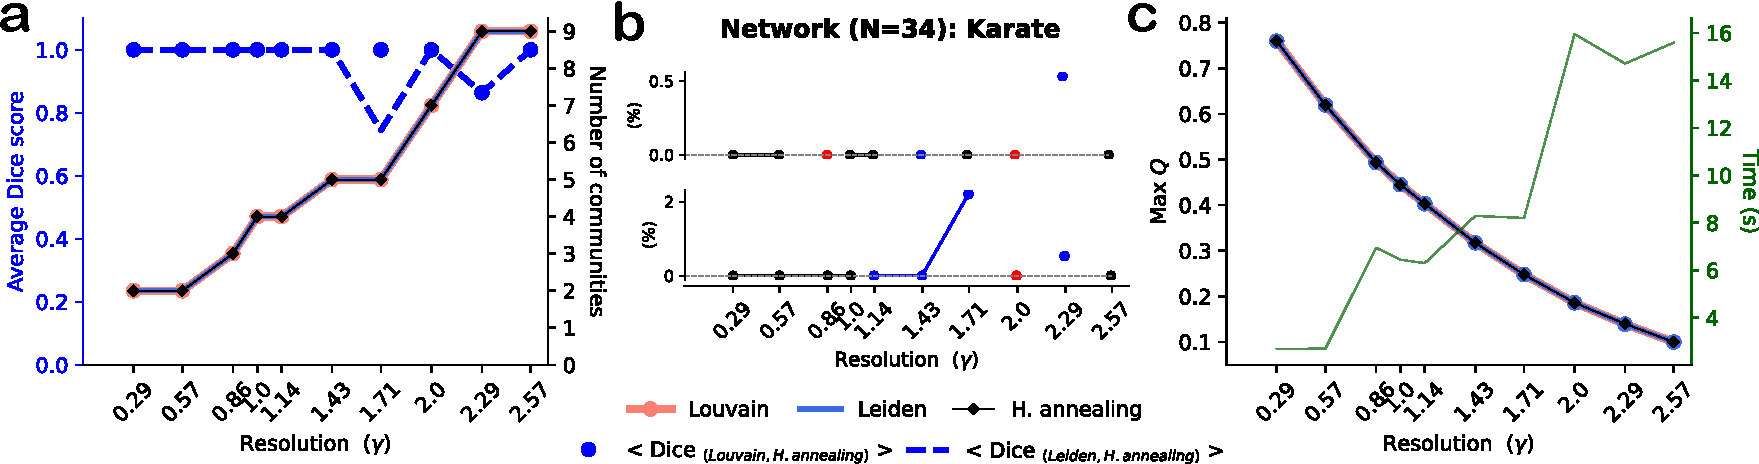
\includegraphics[width=1\linewidth]{Figures/FigS1.pdf}
    \caption{\textbf{Hierarchical annealing in the Karate Club network for different resolution parameters.} \textbf{a} Measure of the average overlap between the communities found by the Louvain and Hierarchical annealing algorithms (left axis, blue) and the number of communities (right axis, salmon and black) as a function of the resolution parameter $\gamma$. \textbf{b} Relative increase of the Hierarchical annealing measured w.r.t. the Louvain (top) and Leiden (bottom) solutions in \textbf{a}. Black, blue, and red symbols depict equal, better, and worse performance of the quantum method respectively. \textbf{c} Maximum modularity per resolution value (left axis, same legend as in \textbf{a}) and the total computing time per solution (right axis, green).}
    \label{fig:resolution_karate}
\end{figure}

\begin{figure}[h]
    \centering
    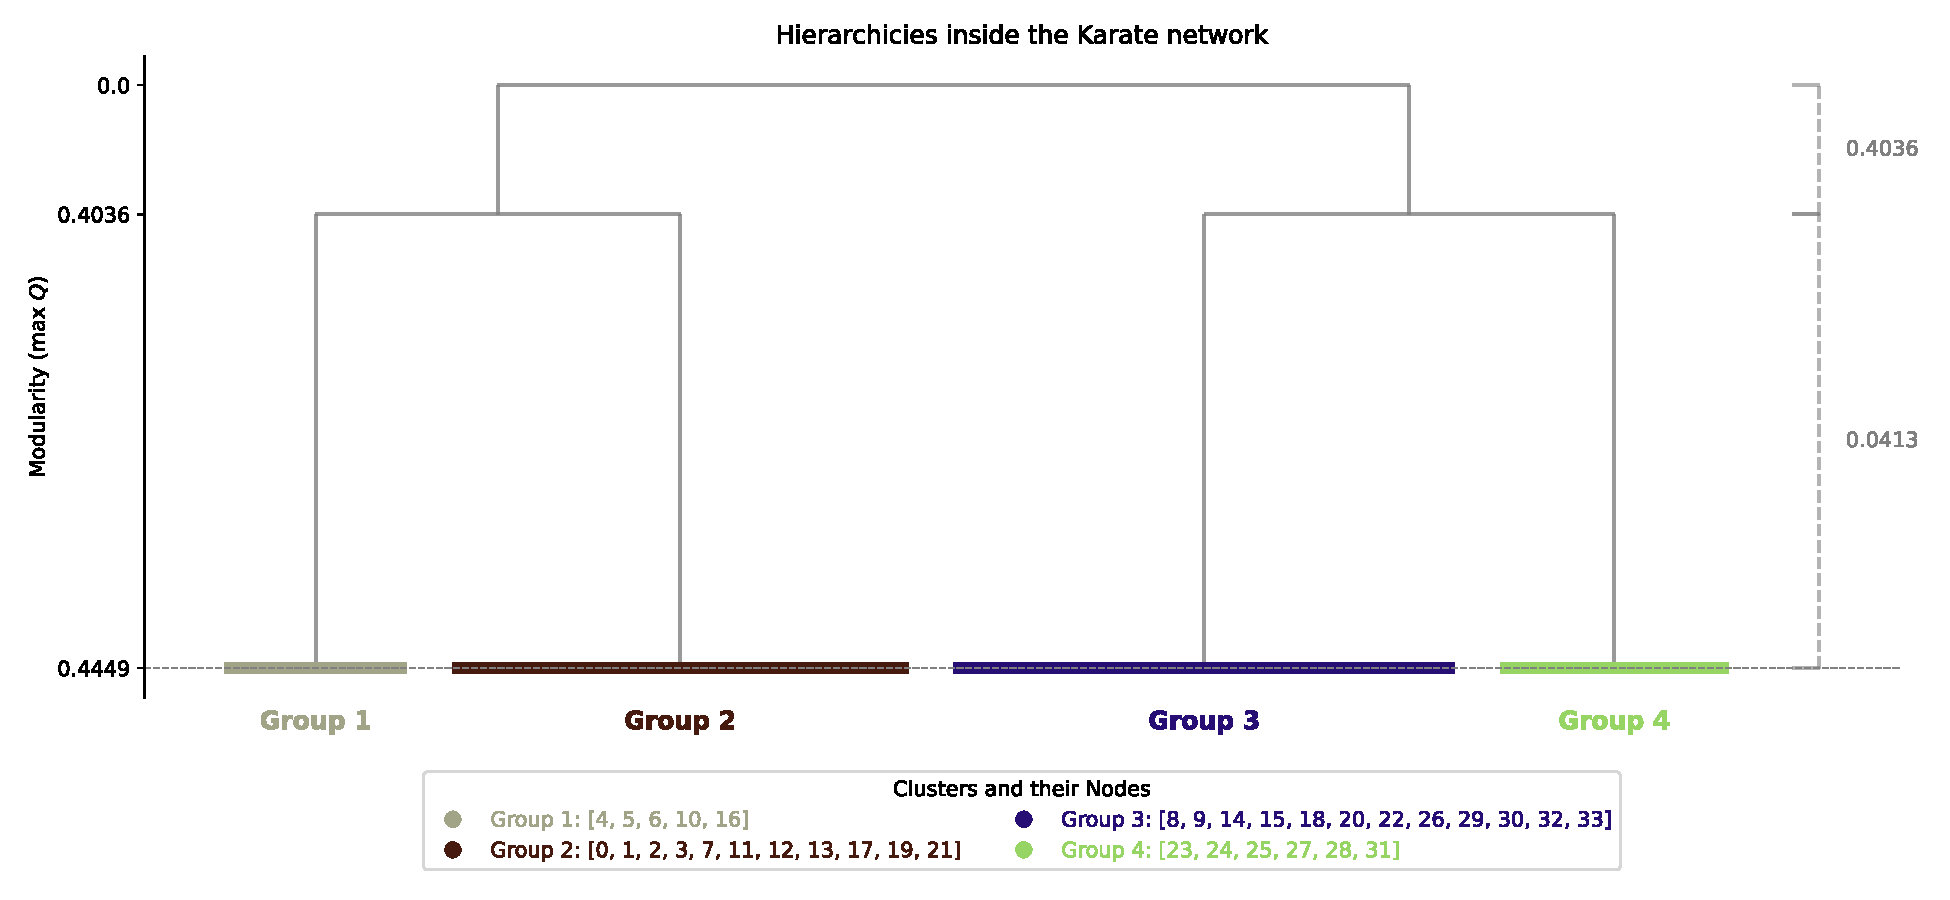
\includegraphics[width=1\linewidth]{Figures/FigS2.pdf}
    \caption{\textbf{Dendrogram of the Karate network \cite{zachary1977information}.} Hierarchical structure found by the H. annealing algorithm. The hierarchy corresponds to the one unraveled after maximizing the modularity of the network as described in the main text; that is, {\tt num\_runs = 50} and {\tt resolution = 1}. The left axis shows the modularity at each step of the process, while the right axis displays the corresponding increments. The bottom-most row represents the final output of the H. annealing algorithm.}
    \label{fig:dendro_karate}
\end{figure}

\begin{figure}[h]
    \centering
    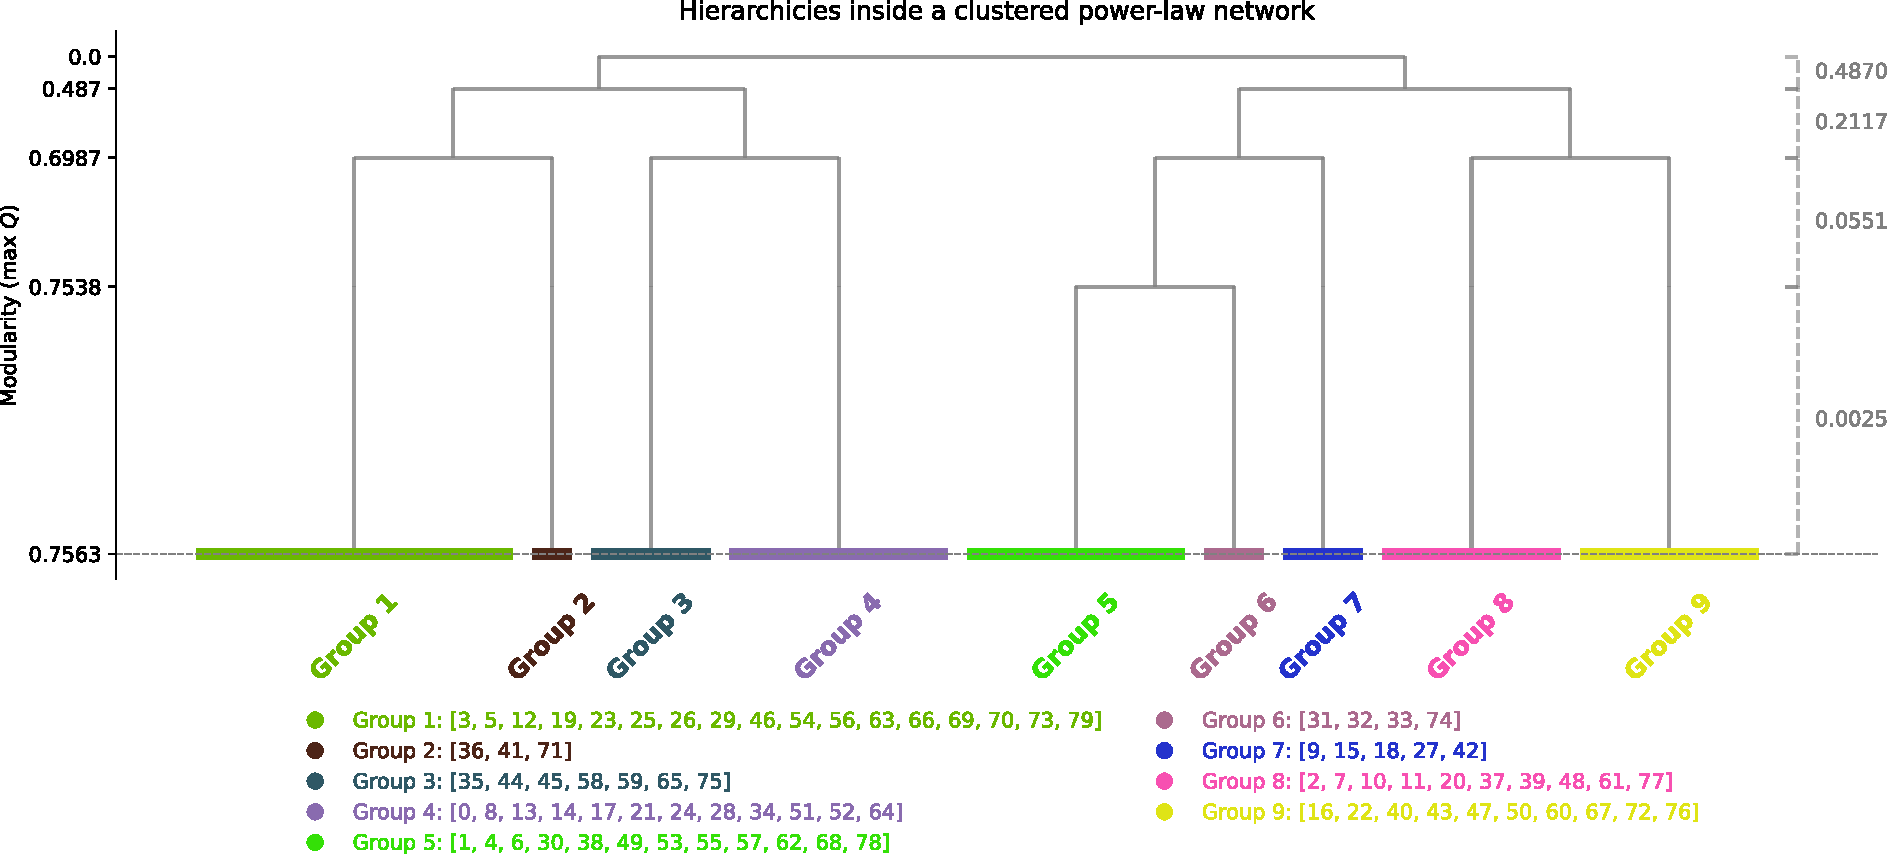
\includegraphics[width=1\linewidth]{Figures/FigS3.pdf}
    \caption{\textbf{Dendrogram of a clustered power-law network \cite{Holme2002} of N=80 nodes.} Hierarchical structure found by the H. annealing algorithm. The hierarchy corresponds to the one unraveled after maximizing the modularity of the network as described in the main text; that is, {\tt num\_runs = 10} and {\tt resolution = 1}. Both the Louvain and Leiden algorithms returned a maximum modularity of $Q=0.7563$. The left axis shows the modularity at each step of the process, while the right axis displays the corresponding increments. The bottom-most row represents the final output of the H. annealing algorithm.}
    \label{fig:dendro_pw_supp}
\end{figure}

\begin{figure}[h]
    \centering
    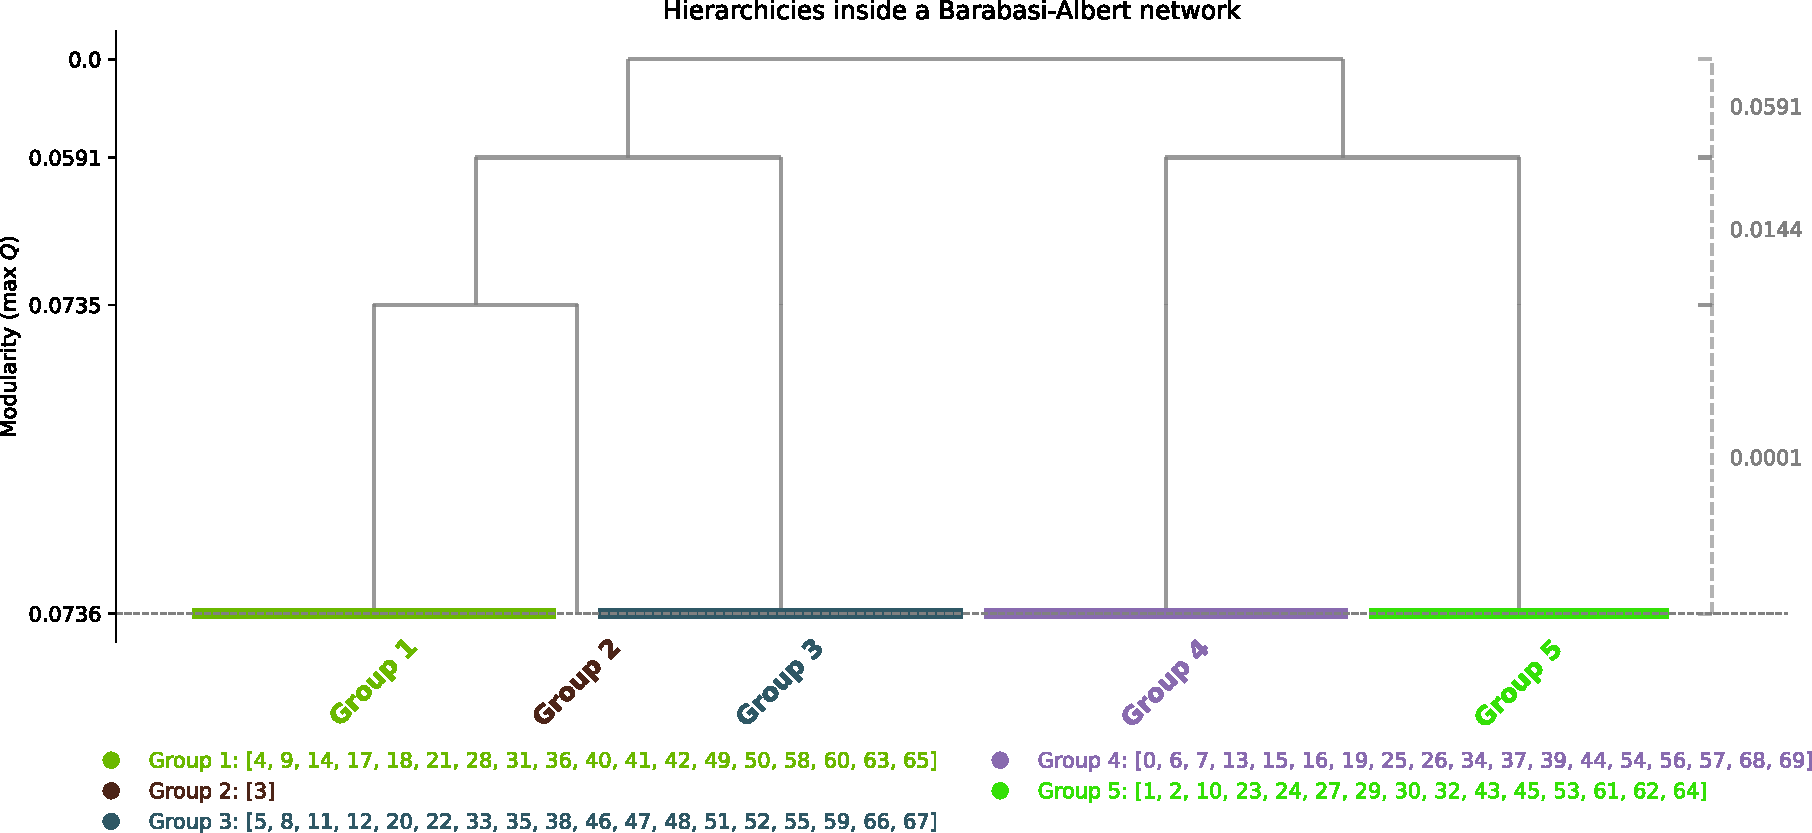
\includegraphics[width=1\linewidth]{Figures/FigS4.pdf}
    \caption{\textbf{Dendrogram of a Barabasi-Albert network \cite{Barabasi1999} of N=70 nodes.} Hierarchical structure found by the H. annealing algorithm. The hierarchy corresponds to the one unraveled after maximizing the modularity of the network as described in the main text; that is, {\tt num\_runs = 20} and {\tt resolution = 1}. The Louvain and Leiden algorithms returned maximum modularities of $Q=0.0760$ and $Q=0.0698$ respectively. The left axis shows the modularity at each step of the process, while the right axis displays the corresponding increments. The bottom-most row represents the final output of the H. annealing algorithm.}
    \label{fig:dendro_ba}
\end{figure}

\begin{figure}[h]
    \centering
    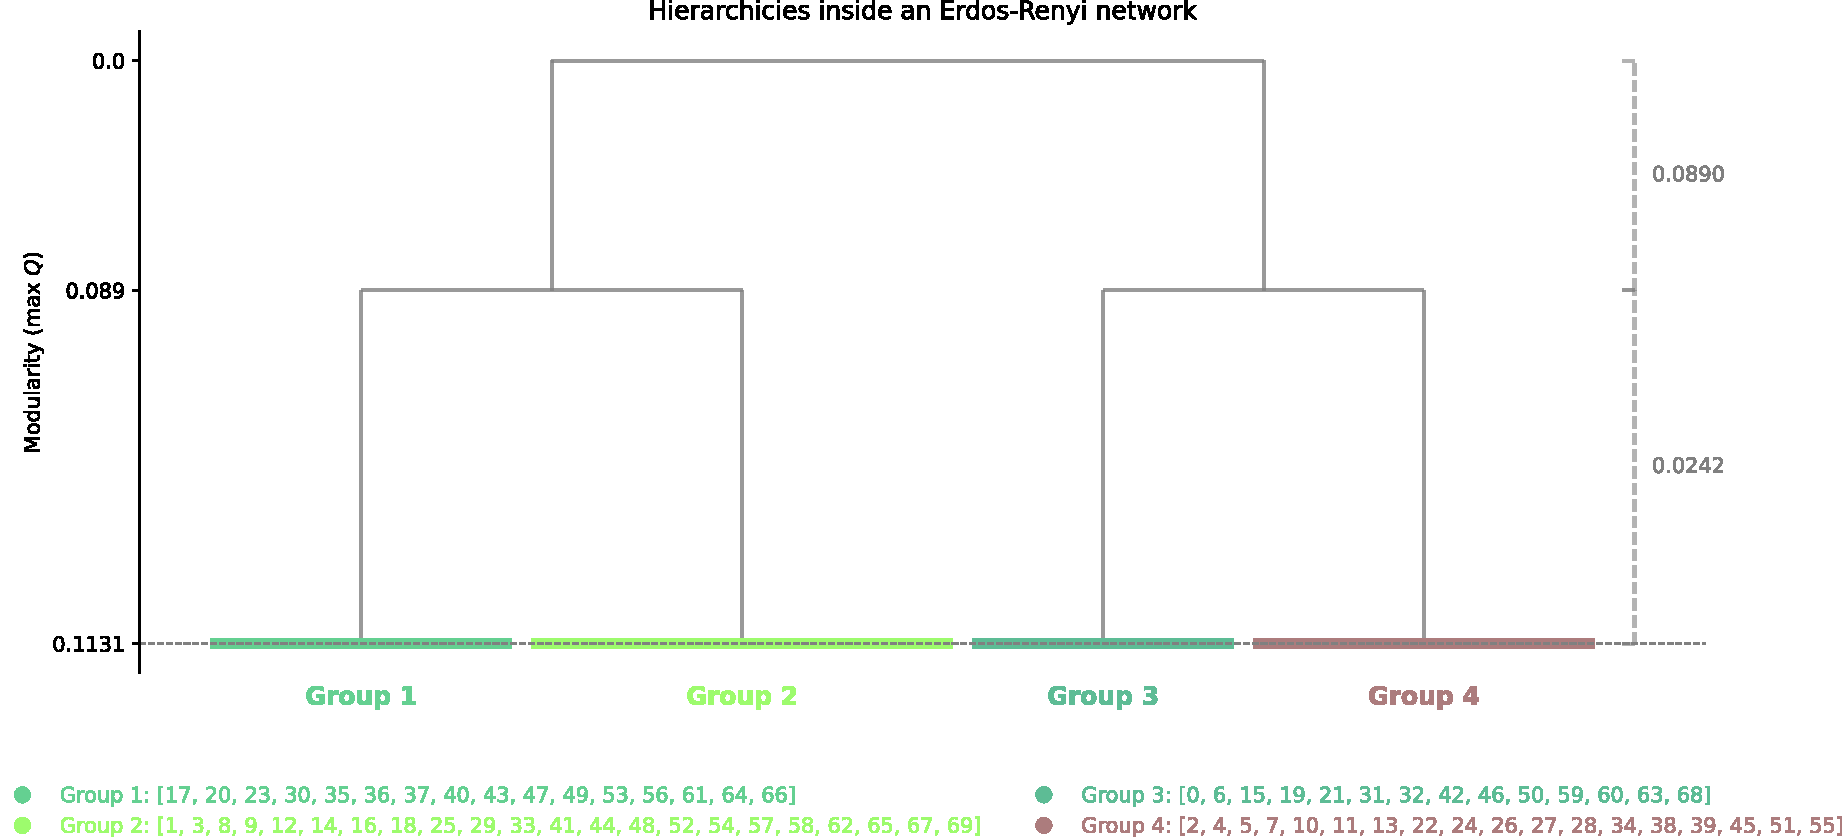
\includegraphics[width=1\linewidth]{Figures/FigS5.pdf}
    \caption{\textbf{Dendrogram of an Erdos-Renyi network \cite{erdds1959random} of N=70 nodes.} Hierarchical structure found by the H. annealing algorithm. The hierarchy corresponds to the one unraveled after maximizing the modularity of the network as described in the main text; that is, {\tt num\_runs = 50} and {\tt resolution = 1}. The Louvain and Leiden algorithms returned maximum modularities of $Q=0.1189$ and $Q=0.1021$ respectively. The left axis shows the modularity at each step of the process, while the right axis displays the corresponding increments. The bottom-most row represents the final output of the H. annealing algorithm.}
    \label{fig:dendro_er}
\end{figure}

\begin{figure}[h]
    \centering
    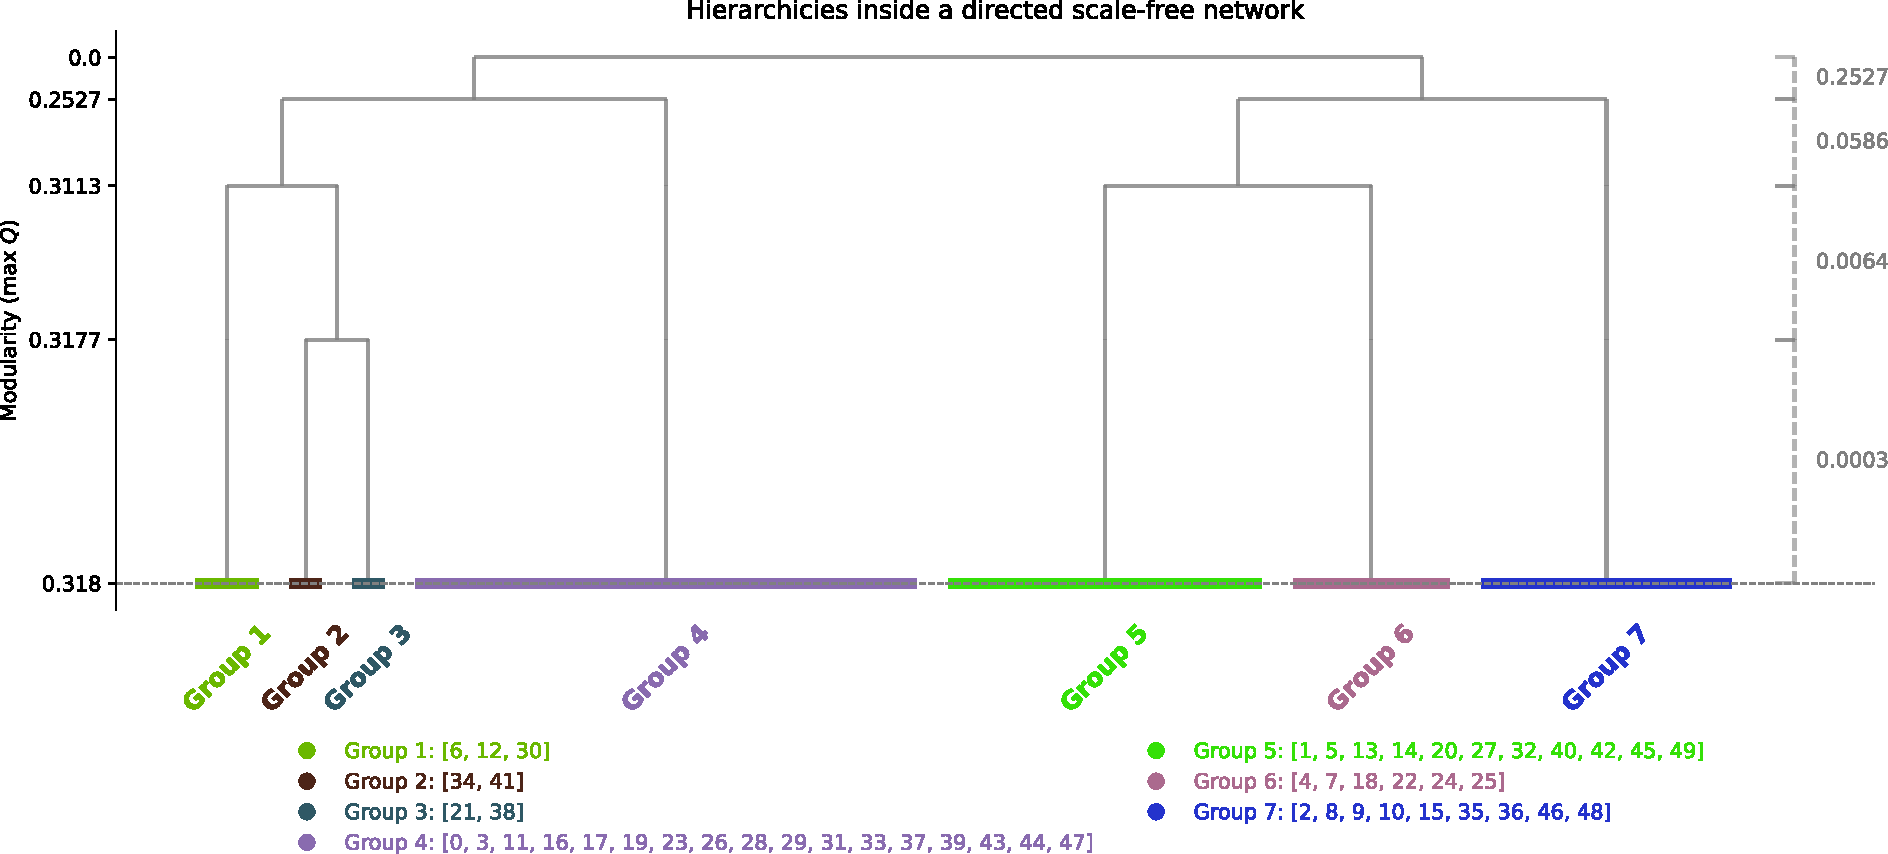
\includegraphics[width=1\linewidth]{Figures/FigS6.pdf}
    \caption{\textbf{Dendrogram of a directed sclae-free network \cite{bollobas2003} of N=50 nodes} Hierarchical structure found by the H. annealing algorithm. The hierarchy corresponds to the one unraveled after maximizing the modularity of the network as described in the main text; that is, {\tt num\_runs = 50} and {\tt resolution = 1}. Both the Louvain and Leiden algorithms returned a maximum modularity of $Q=0.31975$.}
    \label{fig:dendro_sf}
\end{figure}

\begin{figure}[h]
    \centering
    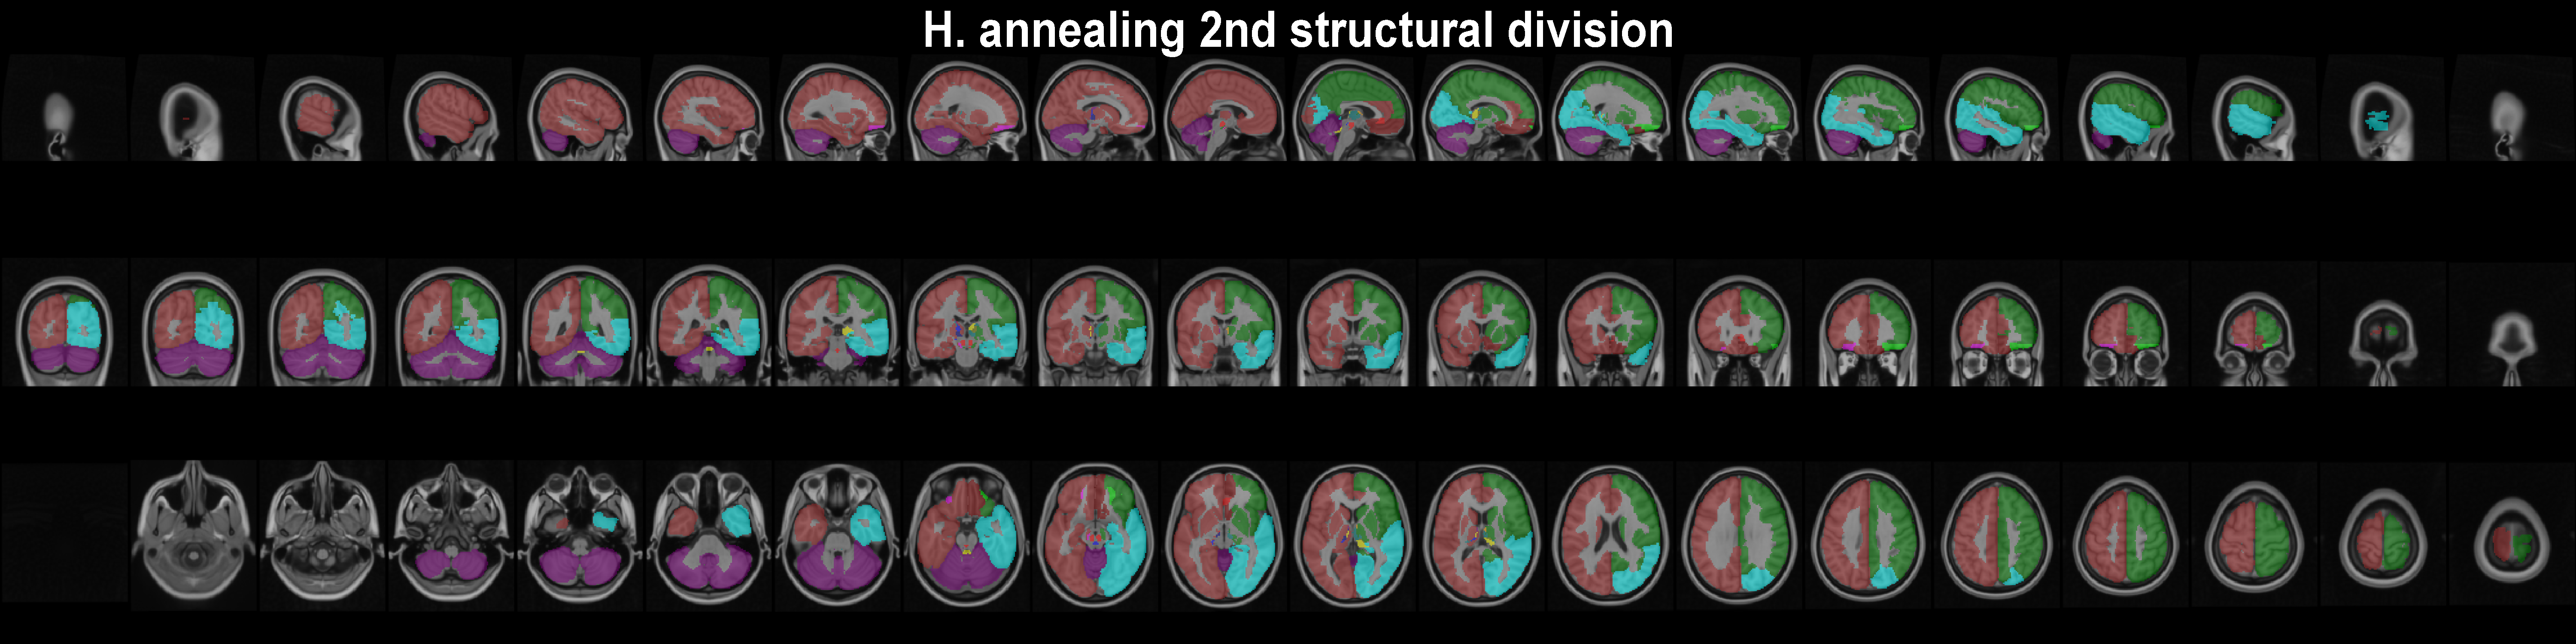
\includegraphics[width=1\linewidth]{Figures/FigS7.pdf}
    \caption{\textbf{Structural communities found at the early steps of the H. annealing process.} We plot the community structure discovered during the 2nd division of the hierarchical method described in the main text. It is visible how the hierarchy carries concise anatomical information, thus being a valid way to inspect hidden structures within complex networks through quantum annealing optimization.}
    \label{fig:hannealing_early_division}
\end{figure}

\begin{figure}[h]
    \centering
    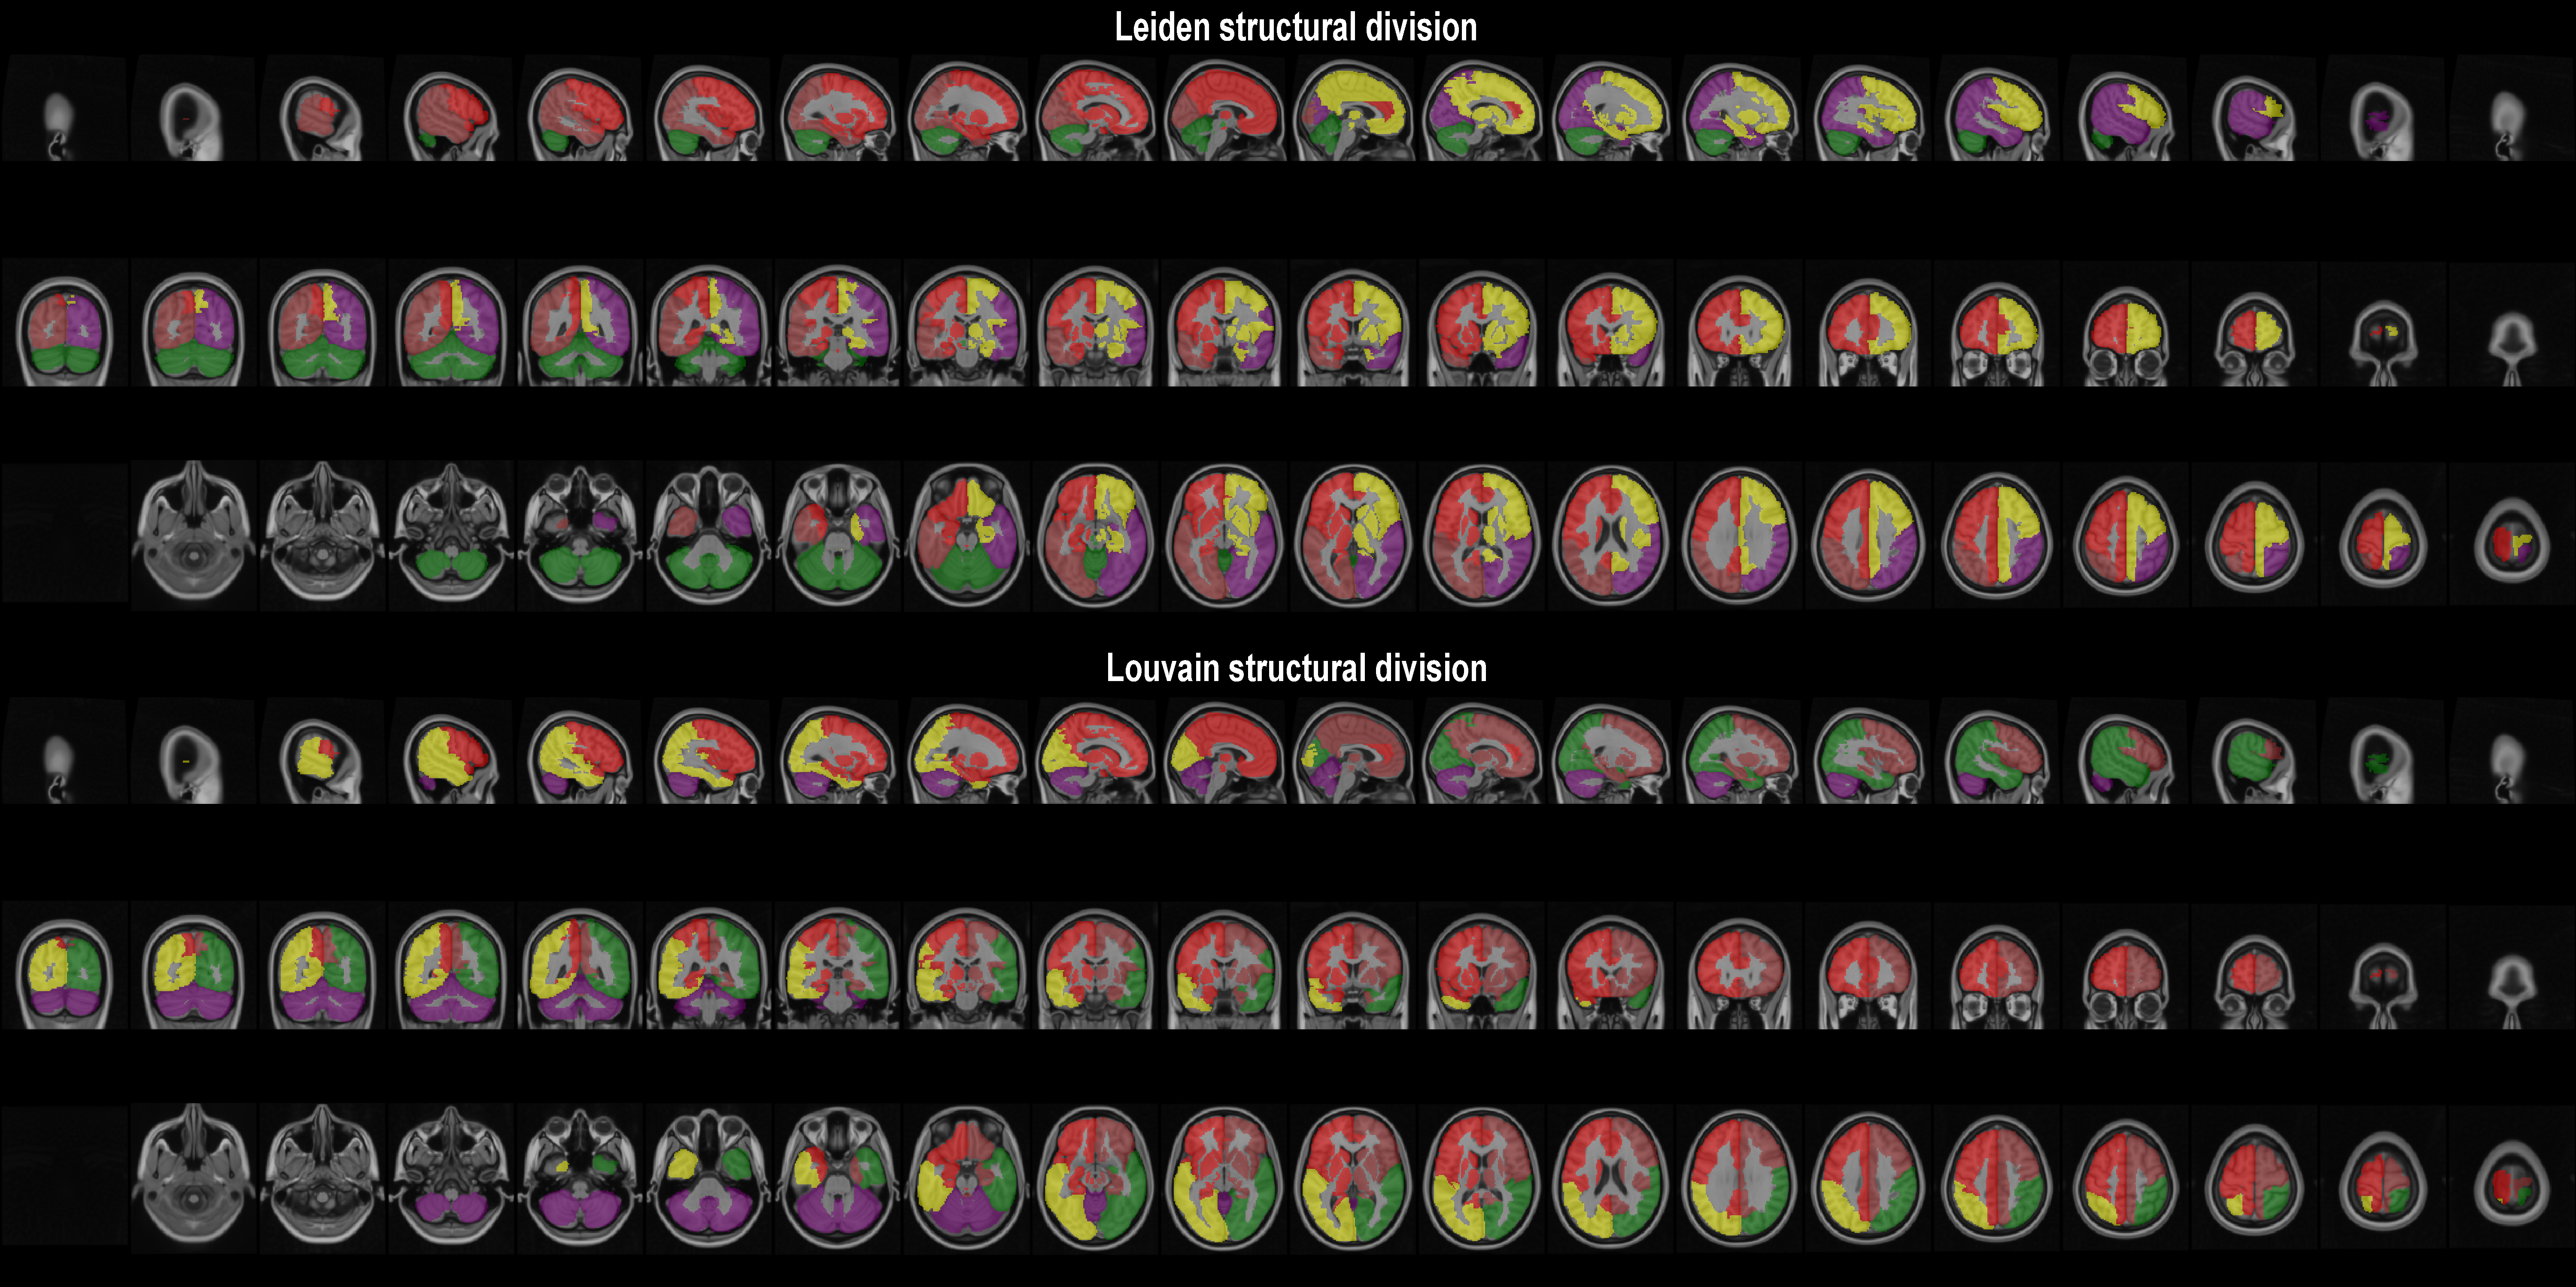
\includegraphics[width=1\linewidth]{Figures/FigS8.pdf}
    \caption{\textbf{Structural communities found by the Leiden and Louvain algorithms.} The resemblance between these communities and the ones found by the annealing process is strikingly high (see main text). The modularity found by the Leiden algorithm was $Q=0.610$, and the modularity returned by the Louvain algorithm was $Q=0.611$.}
    \label{fig:louva_leiden_structural}
\end{figure}

\clearpage
\section*{Software specifics: \textit{Qommunity}}

\subsection*{Architecture}
\begin{figure}[h]
    \centering
    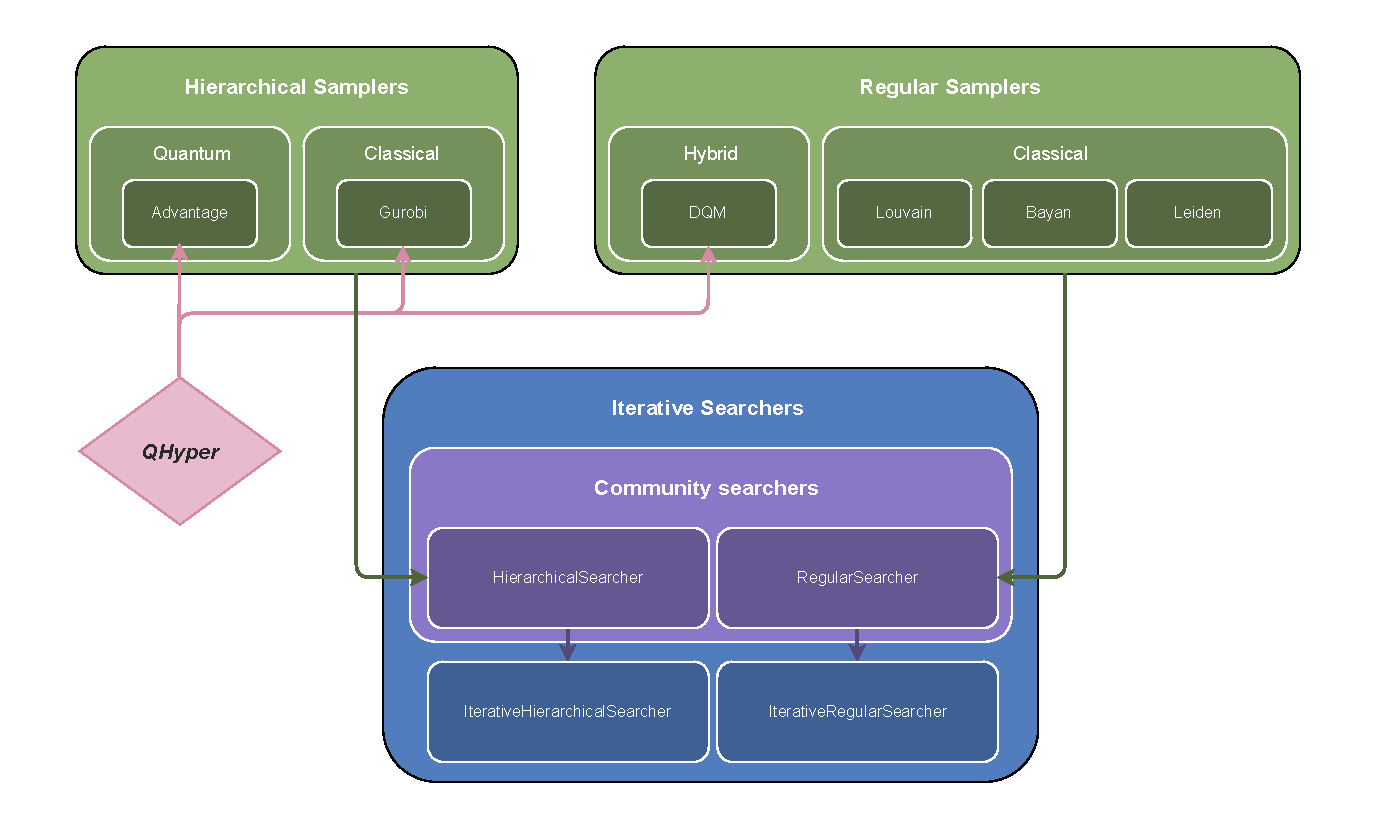
\includegraphics[width=1\linewidth]{Figures/FigS9.pdf}
    \caption{\textbf{Architecture of \textit{Qommunity} library}. The package makes use of the quantum computing library QHyper \cite{lamza_qhyper_2024} to communicate with the quantum annealer using multiple instances of a quadratic binary optimization problem. The Qommunity library also allows the user to choose from several other algorithms and solvers described in the main text. Lastly, the modularity maximization happens at the {\tt IterativeSearcher} class, where any solver and algorithm can be explicitly and automatically run an arbitrary number of times to produce a sufficiently big number of solutions to choose from.}
    \label{fig:qommunity_architecture}
\end{figure}

The \textit{Qommunity} library was designed to integrate several methods for detecting communities in graphs in one place. The implemented methods rely on classical, quantum, and hybrid solutions. The idea was to simplify and standardize the interface for conducting experiments. Several components compartmentalize the architecture, offering user-friendly features: Samplers, Searchers, and IterativeSearchers (Fig. \ref{fig:qommunity_architecture}).

\textit{\textbf{Samplers:}} Through Samplers we specify the method by which we want to detect communities, providing the necessary parameters. Currently, several classical solutions are implemented, such as Gurobi, Louvain \cite{Blondel2008}, Bayan\cite{aref2023}, Leiden \cite{Traag2019}, hybrid -- using DQM \cite{Wierzbinski2023}, and purely quantum -- using Advantage \cite{Johnson2011,lamza_qhyper_2024}. We divided samplers based on how the divisions are done;
\begin{itemize} 
\item regular: the dividing into communities is done according to the algorithms specified inside the Sampler.\item hierarchical: perform binary divisions using classical methods or quantum annealing, depending on the Sampler specified. If no division is optimal, the Sampler returns a single community. Alternatively, each binary division can be further continued in the course of recursion logic provided by the HierarchicalSearcher.
 %binary splits are done, that can be further continued in the course of recursion, if used with the help of a HierarchicalSearcher,
%\item \textcolor{blue}{hierarchical: perform binary splits and are capable of performing optional binary splits, i.e. split only in favour of an optimal solution. The splitting happens as a result of objective function opitimisation or in the course of sampling, depending on the algorithm specified inside the Sampler class},
\end{itemize}

Although Samplers provide community detection methods and can perform the community divisions themselves, the Seacher and IterativeSearcher are the dedicated tools for the user to perform the community detection process comprehensively. 
%To perform community detection with the appropriate Sampler, an instance of it needs to be passed to either the Searcher or the IterativeSearcher.

\textit{\textbf{Searchers:}} Searchers are responsible for executing community detection and for the appropriate postprocessing of its results.  There are two types of Searchers - hierarchical, which accept Samplers that perform hierarchical divisions of communities, and regular, which perform a non-hierarchical, regular community detection method. Each option is defined by the algorithm of choice 
%within the Sampler 
as follows: 
%However, the Searchers full scope of responsibility and action depends on their type:
\begin{itemize}
\item regular: they serve as wrappers for the RegularSampler, facilitating the regular community detection.
\item hierarchical: they extend the scope of action far beyond the RegularSearchers, by implementing the logic of recursion in the hierarchical search.  They build the construct of recursive calls. Its execution results in a tree of binary splits. Similar to RegularSearchers, they also wrap the appropriate Sampler, but with a different purpose - to call the community detection method on HierarchicalSampler on each recursion level and, depending on whether a binary split has occurred as its result, decide whether to proceed with recursion. Hence, they build and oversee the process of hierarchical community detection search, described in Algorithm 1 in the Main text.

The hierarchical searchers track the trace of the hierarchical divisions and, if specified by the user, can return it as a division tree, alongside division modularities, corresponding to each hierarchy division level.
\end{itemize}

\textit{\textbf{Iterative Searchers:}}  Iterative Searchers serve as wrappers for community Searchers, responsible for calling their corresponding (i.e. regular or hierarchical) community search method a given number of times. These multiple calls are useful due to the stochastic and probabilistic natures of the algorithms \textit{Qommunity} provides.
As a result, for each iteration, we get a graph divided into communities, its modularity measure, and the execution time. The result may also contain the division trees and the division modularities, in the case of hierarchical community search. Iterative Searchers are used to simplify the execution of experiments aimed at maximizing the modularity of a given network (see Algorithm 2 in the Main text).

\subsection*{High-level Python code examples to use the quantum resources for modularity maximization and interpretation}
\begin{lstlisting}[language=Python, caption=Modularity maximization and community detection using \textit{Qommunity}. After importing the relevant Python modules maximizing the modularity of the network using quantum computing would be trivial., label=python1]
import networkx as nx # Hagberg, et al. 2008
import numpy as np

## ORIGINAL FROM THIS WORK
from Qommunity.samplers.hierarchical.advantage_sampler import AdvantageSampler # H. Annealing
from Qommunity.samplers.hierarchical.gurobi_sampler import GurobiSampler # H. Gurobi

## HYBRID QUANTUM SOLVER (Wierzbinski, et al. 2023)
from Qommunity.samplers.regular.dqm_sampler import DQMSampler 

## ALETERNATIVE BENCHAMRKS
from Qommunity.samplers.regular.bayan_sampler import BayanSampler 
from Qommunity.samplers.regular.leiden_sampler import LeidenSampler
from Qommunity.samplers.regular.louvain_sampler import LouvainSampler

## MODULARITY MAXIMIZATION
from iterative_searcher.iterative_searcher import IterativeSearcher

## NETWORK TO ANALYZE
Graph = nx.karate_club_graph()
# Graph = nx.from_numpy_array(np.genfromtxt("A.csv", delimiter=','))

## PARAMETERS
num_runs = 20
resolution = 1 #

## Initiate the quantum processor and generate the QUBO
adv_sampler = AdvantageSampler(
    Graph, 
    resolution=resolution, 
    num_reads=100, 
    use_clique_embedding=True
)
adv_iterative= IterativeSearcher(adv_sampler)
communities, modularities, times = adv_iterative.run(num_runs=num_runs, save_results=False)

# Only the community with the highest modularity
community_structure = communities[modularities.argmax()]
modularity = modularities.max()
elapsed_time = times[modularities.argmax()]

\end{lstlisting}

\begin{lstlisting}[language=Python, caption=Example to obtain the hierarchical structure of a given network using modularity maximization., label=python2]
import networkx as nx
import numpy as np
import matplotlib.pylab as plt

## IMPORT THE RELEVANT MODULES
from Qommunity.samplers.hierarchical.advantage_sampler import AdvantageSampler
from iterative_searcher.iterative_searcher import IterativeSearcher
from dendro import Dendrogram

## PARAMETERS
num_runs = 20
resolution = 1

## NETWORK
G = nx.karate_club_graph()
# Graph = nx.from_numpy_array(np.genfromtxt("A.csv", delimiter=','))

# COMMUNITY DETECTION USING RECUSRIVE QUANTUM ANNEALING
searcher = IterativeSearcher(
    AdvantageSampler(
        G, 
        resolution=resolution, 
        num_reads=100, 
        use_clique_embedding=True
    )
)
results = searcher.run_with_sampleset_info(num_runs=num_runs, save_results=False, saving_path=None, iterative_verbosity=0)

## MODULARITY MAXIMIZATION (Algorithm 2 in the main Methods)
mods_Adv = results.modularity
communities = results.communities[mods_Adv.argmax()]
division_tree = results.division_tree[mods_Adv.argmax()]
division_modularities = results.division_modularities[mods_Adv.argmax()]
time = results.time[mods_Adv.argmax()]

## PLOTTING AND CUSTOMIZING THE HIERARCHY PLOT
dendro = Dendrogram(G, communities, division_modularities, division_tree)
fig, ax = plt.subplots(1,1,figsize=(13,6))
dendro.draw(
    display_leafs=False,
    yaxis_abs_log=True,
    ax=ax,
    fig=fig,
    communities_labels=["Group 1", "Group 2", "Group 3", "Group 4", "Group 5", "Group 6", "Group 7", "Group 8"],
    fig_saving_path="./Karate/dendrogram.svg",
    title='Hierarchicies inside the Karate network'
)
\end{lstlisting}

%%=============================================%%
%% For submissions to Nature Portfolio Journals %%
%% please use the heading ``Extended Data''.   %%
%%=============================================%%

%%=============================================================%%
%% Sample for another appendix section			       %%
%%=============================================================%%

%% \section{Example of another appendix section}\label{secA2}%
%% Appendices may be used for helpful, supporting or essential material that would otherwise 
%% clutter, break up or be distracting to the text. Appendices can consist of sections, figures, 
%% tables and equations etc.


%%===========================================================================================%%
%% If you are submitting to one of the Nature Portfolio journals, using the eJP submission   %%
%% system, please include the references within the manuscript file itself. You may do this  %%
%% by copying the reference list from your .bbl file, paste it into the main manuscript .tex %%
%% file, and delete the associated \verb+\bibliography+ commands.                            %%
%%===========================================================================================%%

\end{document}
